%
% LaTeX template for prepartion of submissions to PLDI'16
%
% Requires temporary version of sigplanconf style file provided on
% PLDI'16 web site.
%

\documentclass[parskip=half,sigconf,review, anonymous=true, acmcopyrightmode=none]{acmart}
\acmConference[ESEC/FSE 2017]{11th Joint Meeting of the European Software Engineering Conference and the ACM SIGSOFT Symposium on the Foundations of Software Engineering}{4--8 September, 2017}{Paderborn, Germany}

%\documentclass[preprint,numbers,nocopyrightspace,10pt]{sigplanconf}
% \documentclass[pldi-cameraready]{sigplanconf-pldi16}

%
% the following standard packages may be helpful, but are not required
%
%\usepackage{SIunits}            % typset units correctly
\usepackage{courier}            % standard fixed width font
\usepackage[scaled]{helvet} % see www.ctan.org/get/macros/latex/required/psnfss/psnfss2e.pdf
\usepackage{url}                  % format URLs
\urlstyle{same}                   % URL use same font as regular text
                                  %   (regular font is less wide than tt)
\usepackage{listings}          % format code
\usepackage{enumitem}      % adjust spacing in enums
%\usepackage[colorlinks=true,allcolors=blue,breaklinks,draft=false]{hyperref}   % hyperlinks, including DOIs and URLs in bibliography
% known bug: http://tex.stackexchange.com/questions/1522/pdfendlink-ended-up-in-different-nesting-level-than-pdfstartlink

\usepackage[shortcuts]{extdash} % hyphenation, see http://stackoverflow.com/questions/2193307/how-do-i-get-latex-to-hyphenate-a-word-that-contains-a-dash#8649145

\usepackage[normalem]{ulem}
%\usepackage{amsmath}
\usepackage{calc}
\usepackage{algorithm}
\usepackage[noend]{algpseudocode}
\usepackage[T1]{fontenc}
\usepackage{listings}
\usepackage{color}
\usepackage{xspace}
\usepackage{array}
\usepackage{multirow}
\usepackage{varwidth}
\usepackage{tabularx}  % for 'tabularx' environment and 'X' column type
\usepackage{ragged2e}  % for '\RaggedRight' macro (allows hyphenation)
\usepackage{xcolor,colortbl}
\usepackage{graphicx}
\usepackage{mathpartir}

\usepackage{booktabs}
\usepackage{subfig}
%\usepackage[T1]{fontenc}
%\usepackage[ngerman]{babel}
%\usepackage[latin9]{inputenc}
%\usepackage{blindtext}


\newcommand{\doi}[1]{doi:~\href{http://dx.doi.org/#1}{\Hurl{#1}}}   % print a hyperlinked DOI

\newcommand{\cutthree}[1]{}

\newcommand\crule[3][black]{\textcolor{#1}{\rule{#2}{#3}}}

\makeatletter

\renewcommand\paragraph{\@startsection{paragraph}{4}{\z@}%
  {-.5\baselineskip \@plus -2\p@ \@minus -.2\p@}%
  {-3.5\p@}%
  {\bfseries\@parfont}}

\makeatletter

%\newcommand{\todo}[1]{}
%\renewcommand{\todo}[1]{{\color{red} TODO: {#1}}}
\newcolumntype{C}[1]{>{\centering}m{#1}}
%\newcolumntype{C}[1]{>{\centering\let\newline\\\arraybackslash\hspace{0pt}}m{#1}}

\newcommand{\ADComment}[1]{\textcolor{green}{AD: #1}}
%\newcommand{\TSComment}[1]{\textcolor{blue}{TS: #1}}
\newcommand{\HEComment}[1]{\textcolor{orange}{HE: #1}}
%\newcommand{\COULDCUT}[1]{\textcolor{blue}{#1}}
\newcommand{\TSComment}[1]{\textcolor{purple}{TS: #1}}

\newcommand{\KC}{\mathit{KC}}

\newcommand{\kernelmerge}{\textsc{KernelMerge}}

\newcommand{\myfig}{Fig.~}
\newcommand{\myfiglong}{Figure~}
\newcommand{\myfigs}{Figs.~}
\newcommand{\mytab}{Tab.~}
\newcommand{\mytablong}{Table~}
\newcommand{\mysec}{Sec.~}
\newcommand{\myalg}{Alg.~}
\newcommand{\nvidia}{Nvidia\xspace}
\newcommand{\totalcombinations}{70\xspace}
\newcommand{\positivecombinations}{55\xspace}
\newcommand{\cbedot}{\emph{cbe-dot}\xspace}
\newcommand{\cbeht}{\emph{cbe-ht}\xspace}
\newcommand{\ctoctree}{\emph{ct-octree}\xspace}
\newcommand{\tpotm}{\emph{tpo-tm}\xspace}
\newcommand{\sdkred}{\emph{sdk-red}\xspace}
\newcommand{\sdkrednf}{\emph{sdk-red-nf}\xspace}
\newcommand{\lsbh}{\emph{ls-bh}\xspace}
\newcommand{\lsbhnf}{\emph{ls-bh-nf}\xspace}
\newcommand{\cubscan}{\emph{cub-scan}\xspace}
\newcommand{\cubscannf}{\emph{cub-scan-nf}\xspace}
\newcommand{\heuristiccombinations}{eight\xspace}
\newcommand{\effectivethreshold}{5\%\xspace}
\definecolor{Gray3}{gray}{0.9}
\definecolor{Gray2}{gray}{0.75}
\definecolor{Gray1}{gray}{0.6}

% lstlisting macros
\lstset{
  language=C, % choose the language of the code
  showspaces=false, % show spaces adding particular underscores
  showstringspaces=false, % underline spaces within strings
  showtabs=false, % show tabs within strings adding particular underscores
  tabsize=8, % sets default tabsize to 2 spaces
  captionpos=b, % sets the caption-position to bottom
  mathescape=true, % activates special behaviour of the dollar sign
  basicstyle=\footnotesize\tt,
  columns=fullfelxible,
  xleftmargin=2em,
  %commentstyle=\rmfamily\itshape,
  morekeywords={barrier,kernel,global,__device__,__syncthreads,__global__,bool,then,transmit},
  escapeinside={(*@}{@*)},
  numbers=left
}

\newcommand{\transmit}{\mathsf{transmit}}


\newcommand{\code}[1]{\lstset{basicstyle=\tt}\lstinline!#1!\lstset{basicstyle=\scriptsize\tt}}

\newcommand{\MP}{\textsf{MP}}
\newcommand{\LB}{\textsf{LB}}
\newcommand{\SB}{\textsf{SB}}
\newcommand{\noisethreshold}{3\xspace}
\newcommand{\TotalLitmusTests}{196.6\xspace}
\newcommand{\loadop}{\textsf{ld}\xspace}
\newcommand{\storeop}{\textsf{st}\xspace}

\newcommand{\Td}[2]{{#1}_{#2}}
\newcommand{\Tdl}[3]{\langle \Td{#1}{#2}, #3 \rangle}
\newcommand{\Tdlsigma}[4]{\Tdl{#1}{#2}{#4@#3}}

\newcommand{\randstrsolo}{\emph{rand-str}\xspace}
\newcommand{\sysstrsolo}{\emph{sys-str}\xspace}
\newcommand{\nostrsolo}{\emph{no-str}\xspace}
\newcommand{\cachestrsolo}{\emph{cache-str}\xspace}

\newcommand{\randstr}[1]{\emph{rand-str}#1}
\newcommand{\sysstr}[1]{\emph{sys-str}#1}
\newcommand{\nostr}[1]{\emph{no-str}#1}
\newcommand{\cachestr}[1]{\emph{cache-str}#1}


\newcommand{\NumGPUs}{seven\xspace}
\newcommand{\NumApplications}{ten\xspace}
\newcommand{\NumApplicationsUnique}{seven\xspace}

\newcommand{\offerfork}{\mathsf{request\_fork}}
\newcommand{\offerkill}{\mathsf{offer\_kill}}
\newcommand{\globalbarrier}{\mathsf{global\_barrier}}
\newcommand{\resizingglobalbarrier}{\mathsf{resizing\_global\_barrier}}
\newcommand{\getgroupid}{\mathsf{get\_group\_id}}
\newcommand{\getnumgroups}{\mathsf{get\_num\_groups}}
\newcommand{\getlocalid}{\mathsf{get\_local\_id}}
\newcommand{\getglobalid}{\mathsf{get\_global\_id}}
\newcommand{\getlocalsize}{\mathsf{get\_local\_size}}
\newcommand{\getglobalsize}{\mathsf{get\_global\_size}}

\newcommand{\keyword}[1]{\mathsf{#1}}

\newcommand{\NumAlgorithms}{8}

\begin{document}

\title{Cooperative Kernels: GPU Multitasking for Blocking Algorithms}

\begin{abstract}
There is growing interest in accelerating irregular data-parallel
algorithms on GPUs.  These algorithms are typically \emph{blocking},
so they require fair scheduling.  But GPU programming models
(e.g.\ OpenCL) do not mandate fair scheduling, and GPU schedulers are
unfair in practice.  Current approaches avoid this issue by exploiting
scheduling quirks of today's GPUs in a manner that does not allow the
GPU to be shared with other workloads (such as graphics rendering
tasks).  We propose \emph{cooperative kernels}, an extension to the
traditional GPU programming model geared towards writing blocking
algorithms.  Workgroups of a cooperative kernel \emph{are} fairly
scheduled, and multitasking is supported via a small set of language
extensions through which the kernel and scheduler cooperate.  We
describe a prototype implementation of a cooperative kernel framework
implemented in OpenCL 2.0 and evaluate our approach by porting a set
of blocking GPU applications to cooperative kernels and examining
their performance under multitasking.  Our prototype exploits no
vendor-specific hardware, driver or compiler support, thus our results
provide a lower-bound on the efficiency with which cooperative kernels
can be implemented in practice.

\end{abstract}


%
% any author declaration will be ignored  when using 'pldi' option (for double blind review)
%

%\authorinfo{}
%{\makebox{} \\
%}
%{}

%\authorinfo{Tyler Sorensen}
%{\makebox{Imperial College London, UK} \\
%}
%{t.sorensen15@imperial.ac.uk}

%\authorinfo{Alastair F. Donaldson}
%{\makebox{Imperial College London, UK} \\
%}
%{alastair.donaldson@imperial.ac.uk}


\maketitle

\newcommand{\myparagraph}[1]{\paragraph{#1}}
%{\noindent{\bf\emph{#1}}\hspace{1em}}

\section{Introduction}\label{sec:intro}

\myparagraph{The needs of irregular data-parallel algorithms}
%Acceleration of general-purpose computations on graphics processing
%units (GPUs) has tended to focus on \emph{regular} data-parallel
%algorithms, for which work to be processed can be evenly split between
%the workgroups that execute a GPU kernel ahead of time.  However,
Many interesting data-parallel algorithms are \emph{irregular}: the amount
of work to be processed is unknown ahead of time and may be determined
by the computation itself.  There is growing interest in accelerating
such algorithms on GPUs, particularly the ones that
traverse and manipulate linked data structures~\cite{owens-persistent,DBLP:conf/ipps/KaleemVPHP16,DBLP:conf/ipps/DavidsonBGO14,DBLP:conf/hipc/HarishN07,DBLP:journals/topc/MerrillGG15,DBLP:conf/egh/VineetHPN09,DBLP:conf/ppopp/NobariCKB12,DBLP:conf/hpcc/SolomonTT10a,DBLP:conf/popl/PrabhuRMH11,DBLP:conf/ppopp/Mendez-LojoBP12,DBLP:conf/oopsla/PaiP16,DBLP:conf/oopsla/SorensenDBGR16,DBLP:conf/egh/CedermanT08,TPO10,BNP12,Pannotia}.

Irregular algorithms usually require \emph{blocking synchronization}
between workgroups, to balance load and communicate intermediate
results.  For example, many graph algorithms employ a level-by-level
strategy, requiring a global barrier between each level, and work
stealing algorithms require each workgroup to maintain a queue, which
is typically protected by a mutex to enable stealing by other
workgroups.

To operate correctly, a blocking concurrent algorithm requires
\emph{fair} scheduling of workgroups.  Without fairness, a
workgroup may fail to make progress, leading to starvation.  For
example, if one workgroup holds a mutex, an unfair scheduler may cause
another workgroup to spin-wait forever for the mutex to be
released.  Similarly, an unfair scheduler can cause a workgroup to spin-wait
indefinitely at a global barrier so that other workgroups do not reach the barrier.

%\vspace{-1mm}
\myparagraph{A degree of fairness: occupancy-bound execution} GPU
schedulers are \emph{not} fair. The current GPU programming
models---OpenCL~\cite{opencl2Spec}, CUDA~\cite{cuda-75} and
HSA~\cite{HSAprogramming11}---specify almost no guarantees regarding
scheduling of workgroups, and current GPU scheduler are unfair in
practice.  Roughly speaking, each workgroup executing a GPU kernel is
mapped to a hardware \emph{compute unit}.\footnote{In practice,
  depending on the kernel, multiple workgroups might map to the same
  compute unit; we ignore this in our current discussion.}
%
The simplest way for a GPU driver to handle more workgroups being
launched than there are compute units is via an \emph{occupancy-bound}
execution
model~\cite{owens-persistent,DBLP:conf/oopsla/SorensenDBGR16} where,
once a workgroup has commenced execution on a compute unit (it has
become \emph{occupant}), the workgroup has exclusive access to the
compute unit until it finishes execution.  Experiments suggest that
the occupancy-bound execution model is widely implemented by today's
GPUs~\cite{owens-persistent,DBLP:conf/oopsla/SorensenDBGR16,DBLP:conf/oopsla/PaiP16,BNP12}.
It is evidently a simple model for device vendors to implement
efficiently.

\begin{figure}[t]
\centering
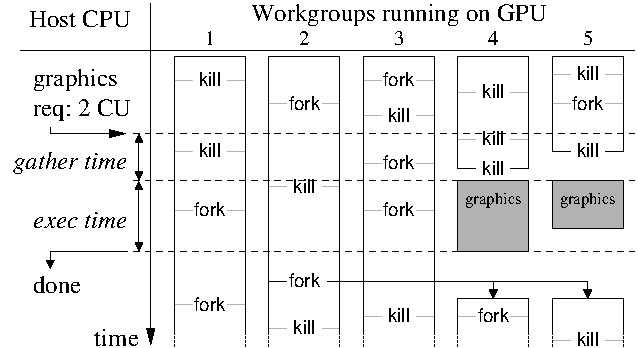
\includegraphics[width=\columnwidth]{overview.pdf}
\caption{Cooperative kernels can flexibly be resized in order to let
other tasks (e.g. graphics) access GPU ressources}
\label{fig:overview}
\end{figure}

The occupancy-bound execution model does not guarantee fair scheduling
between workgroups: if all compute units are occupied then a
not-yet-occupant workgroup will not be scheduled until some occupant
workgroup completes execution.  Yet the execution model \emph{does}
provide fair scheduling between \emph{occupant} workgroups, which are
bound to separate compute units that operate in parallel.  Current GPU
implementations of blocking algorithms assume the occupancy-bound
execution model, which they exploit by launching no more workgroups
than there are available compute units~\cite{owens-persistent}. This
works because \emph{today}'s GPUs seem to provide the occupancy-bound
execution model.

%\vspace{-1mm}
\myparagraph{Resistance to occupancy-bound execution}
Despite its practical prevalence, none of the current GPU programming
models actually mandate occupancy-bound execution.  Further, there are
reasons why this model is undesirable.
% from the point-of-view of
%GPU vendors and end users.
First, the execution model does not enable
multitasking, because a workgroup effectively \emph{owns} a compute
unit until the workgroup has completed execution.  The GPU cannot be used meanwhile for other
tasks, such as graphics rendering.
%Precisely because
%of this problem, operating systems employ a GPU \emph{watchdog} to
%heuristically detect and kill long-running computations on the GPU
%being used for display rendering~\cite{DBLP:conf/iwocl/SorensenD16}.
Second, \emph{energy throttling} is
an important concern for battery-powered devices~\cite{DBLP:journals/comsur/Vallina-RodriguezC13}.  In the future, it will be desirable for a mobile GPU driver to
power down some compute units if the battery level is low.
Implementing energy
throttling would require being able to suspend the execution of a
workgroup, powering down the compute unit to which the workgroup was
bound, something that the occupancy-bound execution model does not allow.

Our assessment, informed by discussions with a number of industrial
practitioners who have been involved in the OpenCL and/or HSA
standardisation efforts
(including~\cite{PersonalCommunicationRichards,PersonalCommunicationHowes}
and various engineers from GPU vendors), is that GPU vendors (1) will
not commit to the occupancy-bound execution model they currently
implement, for the above reasons, yet (2) will not guarantee fair
scheduling due to the runtime cost of preempting workgroups in a fair
manner.  Vendors instead wish to retain the essence of the simple
occupancy-bound model, supporting preemption only in key special
cases.

%\vspace{-1mm}
\myparagraph{Our proposal: cooperative kernels}
%
To summarise: blocking algorithms
demand fair scheduling of workgroups, but for good reasons
GPU vendors will not commit even to the guarantees of the
occupancy-bound execution model.

We propose \emph{cooperative kernels}, an extension to the GPU
programming model that aims to resolve this impasse.  A kernel
that requires fair scheduling is identified as \emph{cooperative}, and written using two additional
language primitives, $\offerkill$ and $\offerfork$, placed by the programmer.

At a point where the cooperative kernel could proceed with fewer
workgroups, a workgroup can execute $\offerkill$, offering to
sacrifice itself to the scheduler.  This indicates that the workgroup
would ideally continue executing, but that the
scheduler may preempt the workgroup; the cooperative kernel
must be prepared to deal with either scenario.
%
At a point where the cooperative kernel could benefit from having
additional workgroups join the computation, a workgroup can execute
$\offerfork$ to indicates that the
kernel is prepared to proceed with the existing set of workgroups, but
is able to benefit from one or more additional workgroups
commencing execution directly after the $\offerfork$ program point.

The use of $\offerfork$ and $\offerkill$ creates a contract between
the scheduler and the cooperative kernel.
Functionally, the
scheduler must guarantee that the workgroups executing a cooperative
kernel are fairly scheduled, while the cooperative kernel must be
robust to workgroups leaving and joining the computation in response
to $\offerkill$ and $\offerfork$.  Non-functionally, a cooperative
kernel must ensure that $\offerkill$ is executed frequently enough
such that the scheduler can accommodate soft-real time constraints,
e.g.\ allowing a smooth frame-rate for graphics, or allowing compute
units to be powered down quickly when required.  The scheduler should
respond to $\offerkill$ and $\offerfork$ calls in a manner that avoids
under-utilisation of hardware resources by the cooperative kernel,
e.g.\ the scheduler should not kill workgroups unless they are
required for another purpose, and should facilitate forking of
additional workgroups when possible.

The cooperative kernels programming model has several appealing
properties:

%\vspace{-1mm}
\begin{enumerate}[leftmargin=*]

\item By providing fair scheduling between workgroups, cooperative
  kernels meet the needs of blocking algorithms, including irregular
  data-parallel algorithms.

\item The model has no impact on the development of regular
  (non-cooperative) compute and graphics kernels: these can be programmed exactly as they
  are now.
%, as can graphics shading routines written using APIs such as
%OpenGL, Vulkan and DirectX.

\item The model is backwards-compatible: if $\offerkill$ and $\offerfork$ are ignored, a cooperative kernel will behave
  exactly as a regular kernel does on current GPUs.

\item Cooperative kernels can be implemented over the occupancy\-/bound
  execution model that current GPUs provide: our prototype implementation requires
  no additional hardware or driver support.  Thus the model should be easy for vendors to implement directly.

\item Our experiments with a range of applications \cutthree{using three GPUs} show that the model can enable efficient multitasking of cooperative and non-cooperative
  tasks.

\end{enumerate}
%\vspace{-1mm}

Placing the new primitives requires manual effort, but our experience porting a representative set of
GPU-accelerated irregular algorithms to use cooperative kernels
(\mysec\ref{sec:portingalgorithms}) suggests that this is straightforward in practice.

In summary, our main contributions are:
\emph{cooperative kernels}, an extended GPU programming model that supports the scheduling requirements of blocking algorithms (\mysec\ref{sec:cooperativekernels}); a \emph{prototype implementation} of cooperative
  kernels on top OpenCL 2.0
  (\mysec\ref{sec:implementation}); and \emph{experiments} assessing the overhead and responsiveness of the cooperative kernels approach over a set of irregular algorithms \cutthree{across three GPUs} (\mysec\ref{sec:experiments}).

We begin by providing background on OpenCL via two motivating examples (\mysec\ref{sec:background}).  At the end we discuss related work (\mysec\ref{sec:relatedwork}) and avenues for future work (\mysec\ref{sec:conclusion}).

\section{Background and Examples}\label{sec:background}

We outline the OpenCL programming model on which we
base cooperative kernels (\mysec\ref{sec:opencl}), and illustrate
OpenCL and the scheduling requirements of irregular algorithms using two examples: a work stealing queue and frontier-based graph traversal
(\mysec\ref{sec:openclexamples}).

\subsection{OpenCL Background}\label{sec:opencl}

% \paragraph{OpenCL concepts}
% An OpenCL program is typically executed by many \emph{threads} running
% in parallel. Threads are organized into \emph{workgroups} of equal
% size. The memory is organized in three levels: \emph{global} memory is
% accessible by any thread, \emph{local} memory is shared at the workgroup
% level (i.e., threads of different workgroups cannot access the same
% local memory), and \emph{private} memory is dedicated to thread-level
% storage and cannot be shared between threads. These concepts are
% illustrated over the two examples.


An OpenCL program is divided into \emph{host} and \emph{device}
components.  A host application runs on the CPU and launches one or
more \emph{kernels} that run on accelerator devices---GPUs in the
context of this paper.  A kernel is written in OpenCL C, based on C99.
All threads executing a kernel start at the same entry function with
identical arguments.  A thread can call $\getglobalid$
to obtain a unique id, to access distinct data or follow different control flow paths.

The threads of a kernel are divided into \emph{workgroups}, each consisting of a fixed number of threads.  Functions
$\getlocalid$ and $\getgroupid$ return a thread's local id within
its workgroup and the id of the workgroup.
%
%\footnote{For simplicity we assume 1D kernels, which captures all the
%irregular algorithms we know of, and write
%e.g.\ $\getglobalid$ for $\getglobalid(0)$.
%}
%
The number
of threads per workgroup and number of workgroups are obtained via
$\getlocalsize$ and $\getnumgroups$.
%A thread's local and global
%id are related by $\getglobalid = \getgroupid \times
%\getlocalsize + \getlocalid$.  The total number of threads executing the
%kernel is given by $\getglobalsize = \getlocalsize \times \getnumgroups$.

Execution of the threads in a workgroup can be synchronised via a
workgroup barrier. This barrier is a \emph{workgroup-level} function:
it can only appear in conditional code if all threads in a workgroup
that reach the barrier agree on the guards of all enclosing
conditional statements.  A \emph{global} barrier (synchronising all
threads of a kernel) is \emph{not} provided as a primitive.

\myparagraph{Memory spaces and memory model} A kernel has access to
four memory spaces.  \emph{Shared virtual memory} (SVM) is accessible
to all device threads and the host concurrently.  \emph{Global} memory is
shared among all device threads.  Each workgroup has a
portion of \emph{local} memory for fast intra-workgroup communication.
Every thread has a portion of very fast \emph{private} memory for
function-local variables.

Communication within a workgroup can be achieved
using a workgroup barrier.  Finer-grained
communication within a workgroup, as well as inter-workgroup
communication and communication with the host while the kernel is
running, is enabled by a set of atomic data types and operations.  In
particular, fine-grained host/device communication is via atomic
operations on SVM.

\myparagraph{Execution model}
OpenCL specifically makes no guarantees about fair scheduling between
workgroups executing the same kernel, stating~\cite[p.\ 31]{opencl2Spec}: \emph{``A
  conforming implementation may choose to serialize the workgroups
%so
%  a correct algorithm cannot assume that workgroups will execute in
%  parallel.
\dots There is no safe and portable way to synchronize across
  the independent execution of workgroups since once in the work-pool,
  they can execute in any order.''}  CUDA similarly provides no guarantees~\cite{cuda-75}.
%
HSA provides limited, one-way guarantees,
stating~\cite[p. 46]{HSAprogramming11}: \emph{Work-group A can wait
  for values written by work-group B without deadlock provided ... (if) A
  comes after B in work-group flattened ID order}. This is not sufficient to support blocking algorithms that use
mutexes and inter-workgroup barriers, both of which require \emph{symmetric} communication between
threads.


\subsection{Motivating Examples}\label{sec:openclexamples}

\begin{figure}

\begin{lstlisting}
(*@\label{line:wksteal:kernelfunc}@*)kernel work_stealing(global Task * queues) {
(*@\label{line:wksteal:getgroupid}@*)  int queue_id = get_group_id();
(*@\label{line:wksteal:mainloop}@*)  while (more_work(queues)) {
(*@\label{line:wksteal:poporsteal}@*)    Task * t = pop_or_steal(queues, queue_id);
    if (t) {
(*@\label{line:wksteal:processtask}@*)      process_task(t, queues, queue_id);
    }
  }
}
\end{lstlisting}
%\vspace{-2mm}
\caption{An excerpt of a work stealing algorithm in OpenCL}\label{fig:workstealing}
%\vspace{-6mm}
\end{figure}

\begin{figure}

\begin{lstlisting}
kernel graph_app(global graph * g,
                 global nodes * n0, global nodes * n1) {
  int level = 0;
  global nodes * in_nodes = n0;
  global nodes * out_nodes = n1;
  int tid = get_global_id();
  int stride = get_global_size();
(*@\label{line:graph:iterate}@*)  while(in_nodes.size > 0) {
    for (int i = tid; i < nodes.size; i += stride) {
      process_node(g, in_nodes[i], out_nodes, level);
    }
(*@\label{line:graph:swap}@*)    swap(&in_nodes, &out_nodes);
(*@\label{line:graph:gb1}@*)    global_barrier();
(*@\label{line:graph:reset}@*)    reset(out_nodes);
    level++;
(*@\label{line:graph:gb2}@*)    global_barrier();
  }
}
\end{lstlisting}
%\vspace{-2mm}
\caption{An OpenCL graph traversal algorithm}\label{fig:graphsearch}
%\vspace{-2mm}
\end{figure}

\myparagraph{Work stealing example}
%
Work stealing enables dynamic balancing of tasks across several
processing units. It is useful when the number of tasks to be
processed is dynamic, due to one task creating an arbitrary number of
new tasks.  Work stealing has been explored in the context of
GPUs~\cite{DBLP:conf/egh/CedermanT08,TPO10}. Each workgroup has an
associated queue from which it obtains tasks to process, and to which
it stores new tasks. If a workgroup's queue is empty, the workgroup
tries to \emph{steal} a task from another queue.

\myfiglong\ref{fig:workstealing} shows a simplified version of a work
stealing kernel. Each thread receives a pointer to the
task queues, in global memory, initialized by the
host to contain the initial tasks. Each thread identifies
its workgroup via $\getgroupid$
(line~\ref{line:wksteal:getgroupid}), which is used as a queue id to access the relevant task queue. The
$\mathsf{pop\_or\_steal}$ function (line~\ref{line:wksteal:poporsteal})
pops a task from the workgroup's queue or, if the queue is empty,
tries to steal a task from other queues.

% is called by all threads of a workgroup.  Inside
% $\mathsf{pop\_or\_steal}$ only the thread with a local id equal to $0$,
% the \emph{master thread}, tries to pop a
% task from the workgroup's queue, or to steal a task from a different
% queue. The master thread uses local memory inside
% $\mathsf{pop\_or\_steal}$ to ensure that the returned value is valid for
% all threads of its workgroup.

If a task was obtained, then the workgroup processes it
(line~\ref{line:wksteal:processtask}): during this operation, new tasks
may be created and pushed into the workgroup's queue.

Although not depicted here, concurrent accesses to queues inside
$\mathsf{more\_work}$ and $\mathsf{pop\_or\_steal}$ are guarded by a
mutex per queue, implemented using atomic compare and swap operations
on global memory.  The kernel presents two opportunities
for spin-waiting: spinning to obtain a mutex, and spinning in the main
kernel loop to obtain a task.  The algorithm thus depends
on a fair scheduler, which is not guaranteed by current GPU programming models.

\myparagraph{Graph traversal example} \myfiglong\ref{fig:graphsearch} shows the
skeleton of a frontier-based graph traversal algorithm; such algorithms have
been shown to execute efficiently on GPUs~\cite{BNP12,DBLP:conf/oopsla/PaiP16}.
The kernel is
given three arguments in global memory: a graph structure, and two
arrays of graph nodes. Initially, $\keyword{n0}$ contains the
starting nodes to process. Private variable $\keyword{level}$ indicates the frontier level currently being
processed, and $\keyword{in\_nodes}$ and $\keyword{out\_nodes}$ point to
distinct node arrays recording the nodes to be processed during the current and next frontier, respectively.

The application iterates as long as the current frontier contains
nodes to process (line~\ref{line:graph:iterate}). At each frontier,
the nodes to be processed are evenly distributed between
threads through \emph{stride} based processing.
%
In this case, the stride is the total number of threads, obtained via
$\getglobalsize$.  Each thread processes nodes with the following sequence of indices:
\code{$\keyword{tid}$+$\keyword{stride}$*0},
\code{$\keyword{tid}$+$\keyword{stride}$*1},
\code{$\keyword{tid}$+$\keyword{stride}$*2}, etc., where $\keyword{tid}$ is a thread's global id.
A thread processes a node via $\keyword{process\_node}$, which may (a) push nodes to process in the next frontier to
$\keyword{out\_nodes}$ and (b) use the current frontier, $\keyword{level}$, in
the computation. After processing the frontier, the threads swap their
node array pointers (line~\ref{line:graph:swap}).

At this point, the GPU threads must wait for all other threads to
finish processing the frontier. To achieve
this, we use a global barrier construct
(line~\ref{line:graph:gb1}). After all threads reach this point, the
output node array is reset (line~\ref{line:graph:reset}) and the level
is incremented. The threads use another global barrier to wait until the output node is
reset (line~\ref{line:graph:gb2}), after which they continue to the next frontier.

The global barrier used in this application is not provided as a GPU
primitive, though previous works have shown that such a global
barrier can be implemented~\cite{XF10,DBLP:conf/oopsla/SorensenDBGR16},
based on CPU barrier designs~\cite[ch. 17]{HS08}.
 These barriers employ spinning to ensure threads wait at the barrier until all
threads have arrived, which requires fair
scheduling between workgroups.% for the barrier to operate correctly.

The mutexes and barriers used by these two examples appear to run
reliably on current GPUs for kernels that are executed with no more
workgroups than there are compute units.  This is due to the fairness
of the occupancy-bound execution model that current GPUs have been
shown, experimentally, to provide.  But, as discussed in
\mysec\ref{sec:intro}, this model is not endorsed
language standards or vendor implementations, and is unlikely to be respected in the future.
%
In \mysec\ref{sec:programmingguidelines} we show how the work stealing
and graph traversal examples of \myfigs\ref{fig:workstealing} and~\ref{fig:graphsearch} can be
updated to use our cooperative kernels programming model to resolve
the scheduling issue.


\section{Cooperative Kernels}\label{sec:cooperativekernels}

We present our cooperative kernels programming model as an extension
to OpenCL.  However, the cooperative kernels concept is more general,
and could be applied to extend other GPU programming models, such as
CUDA and HSA.  We describe the semantics of the model
(\mysec\ref{sec:semantics}), use our motivating examples to discuss
programmability (\mysec\ref{sec:programmingguidelines}), outline
important nonfunctional properties that the model requires to work
successfully (\mysec\ref{sec:nonfunctional}) and explain that the
model is backwards-compatible
(\mysec\ref{sec:backwardscompatibility}).
%
In Appendices~\ref{appendix:semantics} and~\ref{appendix:semanticalternatives} (supplementary material)
we present a formal semantics for cooperative kernels atop an abstract GPU programming model,
and discuss several cases where we
might have taken different and also reasonable semantic decisions.

\subsection{Semantics of Cooperative Kernels}\label{sec:semantics}

As with a regular OpenCL kernel (see \mysec\ref{sec:opencl}), a
cooperative kernel is launched by the host application.  The host
application passes parameters to the kernel and specifies a desired
number of workgroups, each consisting of a specified number of
threads.  Unlike in a regular kernel, the parameters to a cooperative kernel are immutable (though pointer
parameters can refer to mutable data).

Cooperative kernels are written using the following
extensions: $\transmit$, a qualifier on the variables of a
thread; $\offerkill$ and $\offerfork$, the key functions that enable
cooperative scheduling; and $\globalbarrier$ and $\mathsf{resizing\_global\_}$ $\mathsf{barrier}$
%$\resizingglobalbarrier$
primitives for inter-workgroup synchronisation.

%\vspace{-1mm}
\myparagraph{Transmitted variables}
%
A variable declared in the root scope of the cooperative kernel can
optionally be annotated with a new $\transmit$ qualifier.  Annotating
a variable $v$ with $\transmit$ means that when a workgroup spawns new
workgroups by calling $\offerfork$, the workgroup should transmit its
current value for $v$ to the threads of the new workgroups, to serve
as an initial value for $v$.  We detail the semantics for this when we
describe $\offerfork$ below.

%\vspace{-1mm}
\myparagraph{Active workroups}
%
If the host application launches a cooperative kernel requesting $N$
workgroups, this indicates that the kernel should be executed with a
maximum of $N$ workgroups, and that as many workgroups as possible, up
to this limit, are desired.  However, the scheduler may initially
schedule fewer than $N$ workgroups, and as explained below the number
of workgroups that execute the cooperative kernel can change during
the lifetime of the kernel.

The number of \emph{active workgroups}---workgroups executing the
kernel---is denoted $M$.  Active workgroups
have consecutive ids in the range $[0, M-1]$.
Initially, at least one workgroup is active;
if necessary the scheduler must postpone the kernel until
some compute unit becomes available.

When executed by a cooperative
kernel, $\getnumgroups$ returns $M$, the \emph{current} number of
active workgroups.  This is in contrast to $\getnumgroups$ for
regular kernels, which returns the fixed number of workgroups that
were requested at kernel launch time (see \mysec\ref{sec:opencl}).

Fair scheduling \emph{is} guaranteed between active workgroups;
i.e.\ if some thread in an active workgroup is enabled, then
eventually this thread is guaranteed to execute an instruction.

%Note that our programming model does not mandate that
%threads within a workgroup must be fairly scheduled, and indeed this
%is often not the case in GPU programming models, because threads are
%often organised into \emph{warps} or \emph{wavefronts} within a
%workgroup, exhibiting lock-step predicated execution that is
%inherently unfair.

%\vspace{-1mm}
\myparagraph{Semantics for $\offerkill$}
%
The $\offerkill$ primitive allows the cooperative kernel to return
compute units to the scheduler by offering to sacrifice workgroups.
The idea is as follows: allowing the scheduler to arbitrarily and abruptly terminate execution
of workgroups might be drastic, yet the kernel
may contain specific program points at which a workgroup could
\emph{gracefully} leave the computation.
%We give examples of these
%for work stealing and graph traversal in \mysec\ref{sec:programmingguidelines}.

Similar to the OpenCL workgroup $\mathsf{barrier}$ primitive,
$\offerkill$, is a workgroup-level function---it must be encountered
uniformly by all threads in a workgroup (see
\mysec\ref{sec:opencl}).

Suppose a workgroup with id $m$ executes $\offerkill$.
If the workgroup has the highest largest id of all active workgroups then it can be killed by the scheduler, except that workgroup 0 can never be killed (to ensure that the kernel computation does not terminate early).  More formally, if $m < M-1$
or $M=1$ then $\offerkill$ is a no-op.  If instead $M > 1$ and $m =
M-1$, the scheduler can choose to ignore the offer, so that $\offerkill$
executes as a no-op, or accept the offer, so that execution of the workgroup ceases and
the number of active workgroups $M$ is atomically decremented by one.
%In the second case, the scheduler can assign some other task to
%the compute unit on which the workgroup was executing.


%\vspace{-1mm}
\myparagraph{Semantics for $\offerfork$}
%
Recall that
a desired limit of $N$ workgroups was specified when the cooperative kernel was launched, but that the number of active workgroups, $M$, may be smaller
than $N$, either because (due to competing workloads) the scheduler
did not provide $N$ workgroups initially, or because the kernel has
given up some workgroups via $\offerkill$ calls.  Through the
$\offerfork$ primitive (also a workgroup-level function), the kernel and scheduler can collaborate to allow new
workgroups to join the computation at an appropriate point and with
appropriate state.

Suppose a workgroup with id $m\leq M$ executes $\offerfork$.  Then the following occurs: an
integer $k \in [0, N-M]$ is chosen by the scheduler;
$k$ new workgroups are spawned with consecutive ids in the range $[M,
  M+k-1]$; the active workgroup count $M$ is atomically incremented by $k$.

The $k$ new workgroups commence execution at the program point
immediately following the $\offerfork$ call.  The variables that
describe the state of a thread are all uninitialised for the threads
in the new workgroups; reading from these variables without first
initialising them is an undefined behaviour.  There are two exceptions
to this: (1) because the parameters to a cooperative kernel are
immutable, the new threads have access to these parameters as part of
their local state and can safely read from them; (2) for each variable
$v$ annotated with $\transmit$, every new thread's copy of $v$ is
initialised to the value that thread 0 in workgroup $m$ held for $v$
at the point of the $\offerfork$ call.
%
In effect, thread 0 of the forking workgroup \emph{transmits} the relevant
portion of its local state to the threads of the forked workgroups.

%We discuss in \mysec\ref{sec:semanticalternatives} the rationale for
%having all new threads obtain this local state portion from thread 0,
%as well as our reasons for selecting which variables to transmit via
%annotations rather than transmitting the entire thread state.

Notice that $k=0$ is always a valid choice for the number of
workgroups to be spawned by $\offerfork$, and is guaranteed if $M$
is equal to the workgroup limit $N$.

%\vspace{-1mm}
\myparagraph{Global barriers}
%
Because workgroups of a cooperative kernel are fairly scheduled, so a
global barrier primitive can be provided, and we specify two variants: $\globalbarrier$
and $\resizingglobalbarrier$.

Our $\globalbarrier$ primitive is a kernel-level function: if it
appears in conditional code then it must be reached by \emph{all}
threads executing the cooperative kernel.  On reaching a
$\globalbarrier$, a thread waits until all threads have arrived at
the barrier.  Once all threads have arrived, the threads may proceed
past the barrier with the guarantee that all global memory accesses
issued before the barrier have completed.  The $\globalbarrier$
primitive can be implemented by adapting an inter-workgroup barrier
design, e.g.~\cite{XF10}, to take account of a growing and shrinking number of workgroups, and the atomic operations provided by
the OpenCL 2.0 memory model enable a memory-safe
implementation~\cite{DBLP:conf/oopsla/SorensenDBGR16}.  However, implementing such a barrier is
involved, hence why we include this function as a primitive.

The $\resizingglobalbarrier$ primitive is also a kernel-level
function.  It is identical to $\globalbarrier$, except that it caters
for cooperation with the scheduler: by issuing a
$\resizingglobalbarrier$ the programmer indicates that the cooperative
kernel is prepared to proceed after the barrier with more or fewer workgroups.

When all threads have reached $\resizingglobalbarrier$,
the number of active workgroups, $M$, is atomically set to a new value, $M'$ say, with $0 < M' \leq N$.
If $M' = M$ then the active workgroups remain unchanged.  If $M' < M$, workgroups $[M', M-1]$ are
killed.  If $M' > M$ then $M'-M$ new workgroups join the computation after the barrier,
as if they were forked from workgroup 0.  In particular, the
$\transmit$-annotated local state of thread 0 in workgroup 0 is
transmitted to the threads of the new workgroups.

The semantics of $\resizingglobalbarrier$ can be modelled via calling $\offerfork$ and $\offerkill$
surrounded, and seperated by calls to a $\globalbarrier$.
%
%\lstset{basicstyle=\small\tt,numbers=none}
%\begin{lstlisting}
%  $\globalbarrier()$;  $\offerfork$();
%  $\globalbarrier()$; $\offerkill()$;
%  $\globalbarrier()$;
%\end{lstlisting}
%\lstset{basicstyle=\scriptsize\tt,numbers=left}
%
The enclosing $\globalbarrier$ calls ensure that the change in number
of active workgroups from $M$ to $M'$ occurs entirely within the
resizing barrier, so that from a programmer's perspective, $M$ changes atomically.  The middle $\globalbarrier$ ensures that forking occurs before killing, so that workgroups $[0, \textrm{min}(M, M') - 1]$ are left intact.

Because $\resizingglobalbarrier$ can be implemented as above, we do not regard it \emph{conceptually} as a primitive of our
model.  However, in
\mysec\ref{sec:resizingbarrier} we show how a resizing barrier can be
implemented more efficiently through direct interaction with the scheduler.

\subsection{Programming With Cooperative Kernels}\label{sec:programmingguidelines}

%We discuss the main semantic change induced by our programming
%model---that the number of workgroups executing a kernel varies
%dynamically---and illustrate the new language constructs and the
%impact of this semantic change by adapting the work stealing and graph
%traversal algorithms of \mysec\ref{sec:openclexamples} to use
%cooperative kernels.

\myparagraph{A changing workgroup count} Unlike in regular OpenCL, the
value returned by $\getnumgroups$ is not fixed during the lifetime of
a cooperative kernel: it corresponds to the active group count $M$,
which changes as workgroups execute $\offerkill$, and $\offerfork$.
The value returned by $\getglobalsize$ is similarly subject to change.
A cooperative kernel must thus be written in a manner that is robust
to changes in the values returned by these functions.

In general, their volatility means that use of these functions should
be avoided.  However, the situation is more stable if a cooperative
kernel does not call $\offerkill$ and $\offerfork$ directly, so that
only $\resizingglobalbarrier$ can affect the number of active
workgroups.  Then, at any point during execution, the threads of a
kernel are executing between some pair of resizing barrier calls,
which we call a \emph{resizing barrier interval} (considering the
kernel entry and exit points conceptually to be special cases of
resizing barriers).  The active workgroup count is constant within
each resizing barrier interval, so that $\getnumgroups$ and
$\getglobalsize$ return stable values during such intervals.
%
As we illustrate below for graph traversal, this can be exploited by algorithms that perform strided
data processing.


\myparagraph{Adapting work stealing}
%
In this example there is no state to transmit since a computation is
entirely parameterised by a task, which is retrieved from a queue
located in global memory. With respect to \myfig~\ref{fig:workstealing},
we add $\offerfork$ and $\offerkill$ calls at the start of the main loop
(below line~\ref{line:wksteal:mainloop}) to let a workgroup offer itself
to be killed or forked, respectively, before it processes a task.  Note
that a workgroup may be killed even if its associated task queue is not
empty, since remaining tasks will be stolen by other workgroups. In
addition, since $\offerfork$ may be the entry point of a workgroup, the
queue id must now be computed after it, so we move
line~\ref{line:wksteal:getgroupid} to be placed just before
line~\ref{line:wksteal:poporsteal}. In particular, the queue id cannot
be transmitted since we want a newly spawned workgroup to read its own
queue and not the one of the forking workgroup.

% \begin{figure}
% \begin{lstlisting}
% kernel work_stealing(global Task * queues) {
% (*@\label{line:cwksteal:morework}@*)  while (more_work(queues)) {
% (*@\label{line:cwksteal:offerfork}@*)    offer_fork();
% (*@\label{line:cwksteal:offerkill}@*)    offer_kill();
% (*@\label{line:cwksteal:getgroupid}@*)    int queue_id = get_group_id();
% (*@\label{line:cwksteal:poporsteal}@*)    Task * t = pop_or_steal(queues, queue_id);
%     if (t) {
%       // task processing may create more work
% (*@\label{line:cwksteal:processtask}@*)      process_task(t, queues, queue_id);
%     }
%   }
% }
% \end{lstlisting}
% \caption{Cooperative version of the work stealing kernel of
%   \myfig~\ref{fig:workstealing}, using $\offerfork$ and
%   $\offerkill$}\label{fig:workstealing-cooperative}
% \end{figure}

\myparagraph{Adapting graph traversal}
\myfiglong\ref{fig:cgraphsearch} shows a cooperative version of the
graph traversal kernel of \myfig\ref{fig:graphsearch} from
\mysec\ref{sec:openclexamples}.  On lines~\ref{line:cgraph:resizing1}
and ~\ref{line:cgraph:resizing2}, we change the original global
barriers into a resizing barriers. Several variables are marked to be
transmitted in the case of workgroups joining at the resizing barriers
(lines~\ref{line:cgraph:transmit1}, \ref{line:cgraph:transmit2} and
\ref{line:cgraph:transmit3}): $\keyword{level}$ must be restored so
that new workgroups know which frontier they are processing;
$\keyword{in\_nodes}$ and $\keyword{out\_nodes}$ must be restored so
that new workgroups know which of the node arrays to use for input and
output. Lastly, the static work distribution of the original kernel is
no longer valid in a cooperative kernel. This is because the stride
(which is based on $M$) may change after each resizing barrier
call. To fix this, we re-distribute the work after each resizing
barrier call by recomputing the thread id and stride
(lines~\ref{line:cgraph:rechunking1} and
\ref{line:cgraph:rechunking2}). This example exploits the fact that
the cooperative kernel does not issue $\offerkill$ nor $\offerfork$
directly: the value of $\keyword{stride}$ obtained from
$\getglobalsize$ at line~\ref{line:cgraph:rechunking2} is stable
until the next resizing barrier at line~\ref{line:cgraph:resizing1}.
%and in particular can be safely used inside the $\keyword{for}$ loop.

\begin{figure}

\begin{lstlisting}
kernel graph_app(global graph *g,
                 global nodes *n0, global nodes *n1) {
(*@\label{line:cgraph:transmit1}@*)  transmit int level = 0;
(*@\label{line:cgraph:transmit2}@*)  transmit global nodes *in_nodes = n0;
(*@\label{line:cgraph:transmit3}@*)  transmit global nodes *out_nodes = n1;
  while(in_nodes.size > 0) {
(*@\label{line:cgraph:rechunking1}@*)    int tid = get_global_id();
(*@\label{line:cgraph:rechunking2}@*)    int stride = get_global_size();
    for (int i = tid; i < nodes.size; i += stride) {
      process_node(g, in_nodes[i], out_nodes, level);
    }
    swap(&in_nodes, &out_nodes);
(*@\label{line:cgraph:resizing1}@*)    resizing_global_barrier();
    reset(out_nodes);
    level++;
(*@\label{line:cgraph:resizing2}@*)    resizing_global_barrier();
  }
}
\end{lstlisting}
%\vspace{-2mm}
\caption{Cooperative version of the graph traversal kernel of \myfig\ref{fig:graphsearch}, using a resizing barrier and $\transmit$ annotations}\label{fig:cgraphsearch}
\vspace{-4mm}
\end{figure}

\myparagraph{Patterns for irregular algorithms}
In \mysec\ref{sec:portingalgorithms} we describe the set of irregular GPU algorithms used
in our experiments, which largely captures the irregular blocking
algorithms that are available as open source GPU kernels.  These all
employ either work stealing or operate on graph data structures, and placing our new constructs follows a common, easy-to-follow pattern in each case.
%
The work stealing algorithms have a transactional flavour
and require little or no state to be carried between transactions.  The point at which a workgroup is ready to process a new task is a natural place for $\offerkill$ and $\offerfork$, and few or no $\transmit$ annotations are required.
%
\myfiglong\ref{fig:cgraphsearch} is representative of
most level-by-level graph algorithms.
It is typically the case that on completing a level of
the graph algorithm, the next level could be processed by more or
fewer workgroups, which $\resizingglobalbarrier$
facilitates.  Some level-specific state must be transmitted to new workgroups.

%Our experience is that cooperative kernels are a good
%fit for at least these two classes of irregular algorithms, in part because they inspired the model.


\subsection{Non-Functional Requirements}\label{sec:nonfunctional}

The semantics presented in \mysec\ref{sec:semantics} describe the
behaviours that a developer of a cooperative kernel should be prepared
for.
%
However, the aim of cooperative kernels is to find a balance that
allows \emph{efficient} execution of algorithms that require fair scheduling, and
\emph{responsive} multitasking, so that the GPU can be shared between
cooperative kernels and other shorter tasks with soft real-time constraints.
%
To achieve this balance, an implementation of the cooperative
kernels model, and the programmer of a cooperative kernel, must strive
to meet the following non-functional requirements.

%\paragraph{Sufficient $\offerkill$ calls}

The purpose of $\offerkill$ is to let the scheduler destroy a workgroup
in order to schedule higher-priority tasks.  The scheduler relies on the
cooperative kernel to execute $\offerkill$ sufficiently frequently that
soft real-time constraints of other workloads can be met.
%
Using our work stealing example: a workgroup offers itself to
the scheduler after processing each task.  If tasks are sufficiently
fast to process then the scheduler have ample opportunities to
de-schedule workgroups.  But if tasks are very time-consuming to
process then it might be necessary to rewrite the algorithm so that
tasks are shorter and more numerous, to achieve a higher rate of calls
to $\offerkill$.
%
Getting this non-functional requirement right is GPU- and
application-dependent.  In \mysec\ref{sec:sizingnoncoop} we conduct
experiments to understand the response rate that would be required to
co-schedule graphics rendering with a cooperative kernel, maintaining
a smooth frame rate.

%\paragraph{Sufficient workgroups for the cooperative kernel}

Recall that, on launch, the cooperative kernel requests $N$ workgroups.
The scheduler should thus aim to provide $N$ workgroups if other constraints allow it,
by accepting an $\offerkill$ only if a compute unit is required for another
task, and responding positively to $\offerfork$ calls if compute units are available.

%Our
%implementation (\mysec\ref{sec:implementation}) is as
%generous as possible to the cooperative kernel in this regard.

%These guidelines are not hard-and-fast rules, and e.g.\ a smart scheduler might respond selectively to $\offerkill$
%and $\offerfork$ calls by predicting future high-priority workloads
%based on past workloads.


\subsection{Backwards Compatibility}\label{sec:backwardscompatibility}

Our new model has no effect on the manner in which traditional GPU
workloads (e.g.\ graphics shaders and and regular
data-parallel computational kernels) are programmed.
%
Furthermore, if our cooperative language extensions are
ignored---$\offerkill$ and $\offerfork$ are treated as no-ops,
$\transmit$ annotations are ignored, and $\globalbarrier$ and
$\resizingglobalbarrier$ calls are redirected to an existing global
barrier implementation (so that no resizing occurs in the latter
case)---then a cooperative kernel will behave just like its
non-cooperative counterpart would behave.
%A developer
%for whom today's occupancy-bound execution model suffices can upgrade
%their kernel to a cooperative form and retain backwards-compatibility
%with today's GPU platforms by pre-processing away our language
%extensions.


\section{Prototype Implementation}\label{sec:implementation}

Our vision is that support for cooperative kernels will be integrated
in the runtimes of future GPU implementations of OpenCL, with driver
support for our new primitives.  To experiment with our ideas on
current GPUs, we have developed a prototype that mocks up the required
runtime support via a \emph{megakernel}, and exploits the
occupancy-bound execution model that these GPUs provide to ensure fair
scheduling between workgroups.  We emphasise that an aim of
cooperative kernels is to \emph{avoid} depending on the
occupancy-bound model.  Our prototype exploits this model simply to
allow us to experiment with current GPUs whose proprietary drivers we
cannot change.  We describe the megakernel approach
(\mysec\ref{sec:megakernel}) and detail various aspects of the
scheduler component of our implementation
(\mysec\ref{sec:schedulerimpl}).

\subsection{The megakernel mock up}\label{sec:megakernel}

Instead of multitasking multiple separate kernels, we merge a set of
kernels into a megakernel---a single, monolithic kernel.  The
megakernel is launched with as many workgroups as can be occupant
concurrently.  One workgroup takes the role of scheduler, and the
scheduling logic is embedded as part of the megakernel.  The remaining
workgroups act as a pool of workers.  A worker repeatedly queries the
scheduler to be assigned a task.  A task corresponds to executing a
cooperative or non-cooperative kernel.  In the non-cooperative case,
the workgroup executes the relevant kernel function uninterrupted,
then awaits further work.  In the cooperative case, the workgroup
either starts from the kernel entry point or immediately jumps to a
designated point within the kernel, depending on whether the workgroup
is an initial workgroup of the kernel, or a forked workgroup.  In the
latter case, the new workgroup also receives a struct containing the
values of all relevant $\transmit$-annotated variables.

\myparagraph{Simplifying assumptions}
%
For ease of implementation, our prototype supports multitasking a
single cooperative kernel with a single non-cooperative kernel (though
the non-cooperative kernel can be invoked many times).
%We assume all
%variables declared at the root lexical scope of a cooperative kernel
%are implicitly $\transmit$-annotated.
%this allows our
%implementation to piggy-back on top of Clang (see below) without
%requiring front-end changes.
We require that $\offerkill$, $\offerfork$ and
$\resizingglobalbarrier$ are called from the entry function of a
cooperative kernel.  This allows us to use $\keyword{goto}$ and
$\keyword{return}$ to direct threads into and out of the kernel.  With
these restrictions we can experiment with interesting irregular
algorithms (see \mysec\ref{sec:experiments}).  A non-mock
implementation of cooperative kernels would not use the megakernel
approach, so we do not deem the engineering effort associated with
lifting these restrictions to be worthwhile.

%\myparagraph{Merging kernels}
%
%We have built a tool, \kernelmerge{}, that takes a cooperative kernel
%and a non-cooperative kernel and merges them to produce a megakernel
%with an embedded GPU scheduler.  We implemented \kernelmerge{} using the
%Clang LibTooling framework~\cite{clang}, leveraging recent Clang support
%for OpenCL 2.0~\cite{ClangOpenCL20}.

\subsection{Scheduler design}\label{sec:resizingbarrier}\label{sec:schedulerimpl}

To enable multitasking through cooperative kernels, the runtime (in
our case, the megakernel) must track the state of workgroups,
i.e.\ whether a workgroup is waiting or computing a kernel, maintain
consistent context states for each kernel, e.g.\ tracking the number
of active workgroups, and provide a safe way for these states to be
modified in response to $\offerfork$/$\offerkill$. We discuss these
issues, and describe the implementation of an efficient resizing
barrier. We describe how the scheduler would handle arbitrary
combinations of kernels, though as noted above our current
implementation is restricted to the case of two kernels.

\myparagraph{Scheduler contexts}
%
%When a workgroup executes a kernel (cooperative or otherwise), it must
%be able to query a consistent context to obtain a workgroup id value
%and the
%number of workgroups executing the kernel. For multi-kernel
%kernel execution, we emulate the $\getnumgroups$ and $\getgroupid$
%primitives via a per kernel \emph{context}, which records: the number of active groups $M$ (irrelevant for a non-cooperative kernel), the number of requested groups $N$, and a mapping from the native workgroup id to a new workgroup
%id valid for the kernel.
%
To dynamically manage workgroups executing cooperative kernels, our
framework must track the state of each workgroup and provide a channel
of communication from the scheduler workgroup to workgroups executing
$\offerfork$ and $\offerkill$. To achieve this, we use a
\emph{scheduler context} structure, mapping a primitive workgroup id
the workgroup's status, which is either \emph{available} or the id of
the kernel that the workgroup is currently executing.  The scheduler
can then send cooperative kernels a \emph{resource message},
commanding workgroups to exit at $\offerkill$, or spawn additional
workgroups at $\offerfork$. Thus, the scheduler context needs a
communication channel for each cooperative kernel. We implement the
communication channels using atomic variables in global memory.

\myparagraph{Launching kernels and managing workgroups}
%
To launch a kernel, the host sends a data packet to the GPU scheduler
consisting of: a kernel to execute, the kernel inputs, and a flag
indicating whether the kernel is cooperative. In our implementation,
this host-device communication channel is built using fine-grained SVM
atomics.

On receiving a data packet describing a kernel launch $K$, the GPU
scheduler must decide how to schedule $K$. Suppose $K$ requests $N$
workgroups. The scheduler queries the scheduler context.  If there are
at least $N$ available workgroups, $K$ can be scheduled
immediately. Suppose instead that there are only $N_a < N$ available
workgroups, but a cooperative kernel $K_c$ is executing. The scheduler
can use $K_c$'s channel in the scheduler context to command $K_c$ to
provide $N - N_a$ workgroups via $\offerkill$.  Once $N$ workgroups
are available,
% the scheduler initialises a kernel context $\KC$ for $K$, setting
%the number of active workgroups to $N$ and mapping available
%workgroups (located in the scheduler context) to their new $\KC$
%workgroup ids.
the scheduler then sends $N$ workgroups from the available workgroups
to execute kernel $K$
% with
%kernel context $\KC$.
(If the new kernel $K$ is itself a cooperative kernel, the scheduler
would be free to provide $K$ with fewer than $N$ active workgroups
initially.)

If a cooperative kernel $K_c$ is executing with fewer workgroups than
it initially requested, the scheduler may decide make extra workgroups
available to $K_c$, to be obtained next time $K_c$ calls $\offerfork$.
To do this, the scheduler asynchronously signals $K_c$ through $K_c$'s
channel to indicate the number of workgroups that should join at the
next $\offerfork$ command.  When a workgroup $w$ of $K_c$ subsequently
executes $\offerfork$, thread 0 of $w$ updates the kernel and
scheduler contexts so that the given number of new workgroups are
directed to the program point after the $\offerfork$ call.  This
involves selecting workgroups whose status is \emph{available}, as
well as copying the values of $\transmit$-annotated variables to the
new workgroups.

\myparagraph{Accounting for concurrency}
%
Concurrent calls to $\offerfork$ must be protected by a mutex to avoid
racing on the available workgroups. The same conflict over available
workgroups can occur when launching a new kernel between the scheduler
and a workgroup calling $\offerfork$. Thus, $\offerfork$ is protected
by a mutex, called the \emph{assignment mutex}.
%provided in the scheduler context.

The assignment mutex additionally protects concurrent calls to
$\offerfork$ and $\offerkill$.  On calling $\offerkill$, a workgroup
is only permitted to exit if the scheduler workgroup currently holds
the assignment mutex; that is, the scheduler is trying to obtain work
groups to send to a task.  Conversely, on calling $\offerfork$ a
workgroup can only spawn new workgroups if the scheduler workgroup
does not hold the assignment mutex.  Thus the assignment mutex, only
ever acquired by the scheduling workgroup, \emph{indirectly} provides
mutual exclusion between a pairs of workgroups executing $\offerkill$
and $\offerfork$ concurrently.

Concurrent calls to $\offerkill$ are acceptable because only the
workgroup with the highest id may exit, automatically ensuring mutual
exclusion for exit-related state changes.

\myparagraph{An efficient resizing barrier}
%
In \mysec\ref{sec:semantics}, we defined the semantics of a resizing
barrier in terms of calls to other primitives.  It is possible,
however to implement the resizing barrier with only one call to a
global barrier with $\offerfork$ and $\offerkill$ baked inside.

We consider barriers that use the master/slave model~\cite{XF10}: one
workgroup (master) collects signals from the other workgroups (slaves)
indicating that they have arrived at the barrier and are waiting for a
reply indicating that they may leave the barrier. Once the master has
received a signal from all slaves, it replies with a signal saying that
they may leave.

Incorporating $\offerfork$ and $\offerkill$ into such a barrier is
straight forward. Upon entering the barrier, the slaves first execute
$\offerkill$, possibly exiting. The master then waits for $M$ slaves
(the number of active workgroups), which may decrease due to
$\offerkill$ calls by the slaves, but will not increase. Once the
master observes that $M$ slaves have arrived, it knows that all other
workgroups are waiting to be released. The master executes
$\offerfork$, and the statement immediately following this
$\offerfork$ is a conditional that forces newly spawned workgroups to
join the slaves in waiting to be released. Finally, the master
releases all the slaves: the original slaves and the new slaves that
joined at $\offerfork$.

This barrier implementation is sub-optimal because workgroups only
execute $\offerkill$ once per barrier call and, depending on order of
arrival, it is possible that only one workgroup is killed per barrier
call, preventing the scheduler from gathering workgroups quickly.

We can reduce the gather time by providing a new
$\keyword{query}$ function for cooperative kernels, which returns the
number of workgroups that the scheduler needs to obtain from the
cooperative kernel.
%
%The programmer cannot call $\keyword{query}$ directly; it is
%invoked from within the resizing barrier implementation.
%
A resizing barrier can now be implemented as follows: (1) the master
waits for all slaves to arrive; (2) the master calls $\offerfork$ and
commands the new workgroups to be slaves; (3) the master calls
$\keyword{query}$, obtaining a value $W$; (4) the master releases the
slaves, broadcasting the value $W$ to them; (5) workgroups with ids
larger than $M-W$ spin, calling $\offerkill$ repeatedly until the
scheduler claims them---we know from $\keyword{query}$ that the
scheduler will eventually do so.
We show in
\mysec\ref{sec:responsiveness} that the barrier using $\keyword{query}$ greatly
reduces the gather time in practice.


\section{Applications and Experiments}\label{sec:experiments}

We discuss our experience porting irregular algorithms to cooperative
kernels and describe the GPUs on which we evaluate these applications
(\mysec\ref{sec:portingalgorithms}).  For these GPUs, we report on
experiments to determine non-cooperative workloads that model the
requirements of various graphics rendering tasks
(\mysec\ref{sec:sizingnoncoop}).  We then examine the overhead
associated with moving to cooperative kernels when multitasking is
\emph{not} required (\mysec\ref{sec:overhead}), as well as the
responsiveness and throughput observed when a cooperative kernel is
multi-tasked with non-cooperative workloads
(\mysec\ref{sec:responsiveness}).

To our knowledge, there are no competing methods against which to
meaningfully compare our approach.  We are not aware of any existing
platform that supports multitasking between long-running, fully-occupant
OpenCL kernels.  Very recent \nvidia{} GPUs, to which we do not yet have
access, support preemption for graphics
applications~\cite{PascalWhitepaper}, but our understanding is that this
cannot yet be leveraged from CUDA, and certainly not from OpenCL.


\subsection{Applications and GPUs}\label{sec:portingalgorithms}

\begin{table}[t]
\normalsize
\centering
\begin{tabular}{ l r r r r r r}
App. & barriers & kill & fork & transmit & LoC & inputs\\
\hline
\rowcolor{Gray1}
color & 2 / 2 & 0 & 0 & 4 & 55 & 2\\
\rowcolor{Gray1}
mis & 3 / 3 & 0 & 0 & 0 & 71 & 2\\
\rowcolor{Gray1}
bc & 3 / 6 & 0 & 0 & 3 & 150 & 2\\
\rowcolor{Gray1}
p-sssp & 3 / 3 & 0 & 0 & 0  & 42 & 1\\
\rowcolor{Gray2}
bfs & 2 / 2 & 0 & 0  & 4  & 185 & 2\\
\rowcolor{Gray2}
l-sssp & 2 / 2 & 0 & 0  & 4  & 196 & 2\\
\rowcolor{Gray3}
octree & 0 / 0 & 1 & 1 & 0 & 213 & 1 \\
\rowcolor{Gray3}
game & 0 / 0 & 1 & 1 & 0 & 308 & 1 \\
\end{tabular} \\
%\vspace{.2cm}
\crule[Gray1]{.2cm}{.2cm} Pannotia \hspace{.4cm} \crule[Gray2]{.2cm}{.2cm} Lonestar GPU  \hspace{.4cm}  \crule[Gray3]{.2cm}{.2cm} work stealing
\caption{Blocking GPU applications investigated}
\label{tab:applications}
\vspace{-8mm}
\end{table}

%\begin{table}[t]
%\footnotesize
%\centering
%\begin{tabular}{ l l l l }
%Chip & HD520 & HD5500 & Iris\\
%\hline
%\# CU  & 24 & 24 & 47 \\
%Driver   & 20.19.15.4501 & 10.18.15.4281 & 20.19.15.4463 \\
%Host CPU & i3-6100U & i7-5600U & i3-5157U \\
%\end{tabular}
%\caption{The Intel GPU platforms used in our evaluation}
%\label{tab:chipstested}
%\end{table}

\mytablong\ref{tab:applications} gives an overview of the 8 irregular
algorithms that we ported to cooperative kernels. Among them, 6 are
graph algorithms, based on the Pannotia~\cite{Pannotia} and
Lonestar~\cite{BNP12} GPU application suites, using global barriers.
We indicate how many of the original number of barriers are changed to
resizing barriers, and how many variables need to be transmitted.  In
all cases all barriers were converted, except for bc which contains
barriers deeper in the call stack, a case not supported by our
prototype although these barriers could in principle be converted. The
remaining 2 algorithms are work stealing applications: each required
the addition of $\offerfork$ and $\offerkill$ at the start of the main
loop, and no variables needed to be transmitted.  For all these
examples, the porting to cooperative kernels was similarly
straightforward to the porting illustrated in
\mysec\ref{sec:programmingguidelines}. Most
graph come with 2 different data sets as input, leading to 13
application/input pairs in total.

From the Lonestar suite we omit two applications that use global
barriers: dmr has been shown to be unstable across GPU
vendors~\cite{DBLP:conf/iwocl/SorensenD16}, and mst is trivially
short-running so that it is not interesting for our multitasking
approach.

Our prototype implementation (\mysec\ref{sec:implementation}) requires
two optional features of OpenCL 2.0: SVM fine-grained buffers and SVM
atomics. This rules out evaluation on \nvidia and ARM Mali GPUs at
present, since these vendors do not yet support OpenCL $2.0$,
equivalent functionality is not provided by \nvidia's CUDA. Intel
drivers meet our requirements on Windows, but not on Linux.
%(we
%confirmed this by trying the upstream driver that requires a patched
%Linux kernel).
AMD support SVM atomics only their Kaveri family of
chips and only on Linux.%, requiring to compile the latest driver.

Among the GPUs available to us, four met our requirements: Intel HD
520, HD 5500 and Iris 6100, and AMD Radeon R7.  However, AMD's Linux
drivers for OpenCL suffer from a known defect whereby long-running
kernels lead to unkillable defunct
processes~\cite{amd-defunct-process}. Because of this behaviour, we
could not experiment on AMD platforms.

%and simultaneously obtained alarming results on this platform when
%using SVM atomics: modifying a kernel to include a simple host/device
%handshake through SVM slowed down kernel execution by an order of
%magnitude in some cases.  This behaviour, combined with the defunct
%processes issue, lead us to suspect that the support we require for
%cooperative kernels is not yet mature enough within AMD's drivers,
%which we plan to discuss with engineers at AMD.

We thus ran our experimental campaign on the Intel GPUs. The results
were similar across the GPUs, so for conciseness, we report only on
the Iris 6100 GPU (driver 20.19.15.4463) with a host CPU i3-5157U. The
Iris has a reported 47 compute units. Results for the two other Intel
GPUs are available in supplementary material.


\subsection{Sizing Non-Cooperative Kernels}\label{sec:sizingnoncoop}

Enabling rendering of smooth graphics in parallel with execution of irregular algorithms is an important use case for our approach.  Because our prototype implementation is based on a megakernel that takes over the entire GPU (see \mysec\ref{sec:implementation}), we cannot assess this use case directly.

We devised the following
procedure to determine non-cooperative OpenCL workloads that simulate
the computational intensity of various graphics rendering workloads.
%
We designed a synthetic kernel that occupies all workgroups of a
GPU for a parameterised time period $t$, invoked in an infinite loop by a host application.  We then
searched for a maximum value for $t$ that allowed the
synthetic kernel to execute without having an observable impact on
graphics rendering.  Using the computed value, we
ran the host application for $X$ seconds, measuring the time $Y < X$
dedicated to GPU execution during this period and the number
of kernel launches $n$ that were issued.  We used $X \geq 10$ in all
experiments.  The values $(X-Y)/n$ and $X/n$ estimate the average time
spent using the GPU to render the display between kernel calls and the
period at which the OS requires the GPU for display rendering,
respectively.

We used this approach to measure the GPU availability required for three
types of rendering: \emph{light}, whereby desktop icons are smoothly
emphasised under the mouse pointer; \emph{medium}, whereby window
dragging over the desktop is smoothly animated; and \emph{heavy}, which
requires smooth animation of a WebGL shader in a browser.  For
\emph{heavy} we used WebGL demos from the Chrome
experiments~\cite{chrome-experiments} running
in a recent version of Firefox.

% the Paper Planes\footnote{\url{https://paperplanes.world}} and
% Kaleidoscope\footnote{\url{http://colordodge.com/Kaleidoscope}}
% shaders running in a recent version of Firefox.

% \begin{table}
% \small
% \centering
% \begin{tabular}{ l r r }
% Workload & Duration (ms) & Rate (ms)\\
% \hline
% light & 3 & 70\\
% medium & 3 & 40\\
% heavy & 10 & 40\\
% \end{tabular}
% \caption{Computed estimates of the GPU requirements for three different classes of graphics rendering}
% \label{tab:noncooperativeworkload}
% \end{table}

Our results are the following: light workloads needs to run 3ms every
70ms, medium ones 3ms every 40ms, and heavy ones 10ms every 40ms. For
the medium and heavy workloads, the 40ms period corresponds to graphics
rendering occurring 25 times per second, which coincides with the human
persistence of vision. The 3ms execution duration of both light and
medium configurations indicates that, as expected, GPU computation is
cheaper for basic display rendering compared with rendering that uses
complex shaders. We use these results to guide our evaluation of the
responsiveness of cooperative scheduling in
\mysec\ref{sec:responsiveness}.

% The
% \emph{Duration} and \emph{Rate} columns report values corresponding to
% $(X-Y)/n$ and $X/n$ in the above discussion, respectively.

% \mytablong\ref{tab:noncooperativeworkload} illustrates the data
% computed for the three types of workloads across our GPUs.

\subsection{The Overhead of Cooperative Kernels}\label{sec:overhead}

%%%%%%%%%%%%%%%%%%%%%%%%%%%%%%%%%%%%%%%%%%%%%%%%%%%%%%%%%%%%%%%%%%%%%%%%%%%%%%%
% chip: hd520
% overall -
% geomean: 1.19835906125
% max ('color', 'ecology', 1.749620120141443)
% -----
% barrier
% max - ('color', 'ecology', 1.749620120141443)
% geomean: 1.18027192048
% -----
% workstealing
% max - ('octree', 'NA', 1.4165788173996423)
% geomean: 1.4165788174
% -----
% chip: iris
% overall -
% geomean: 1.07926294253
% max ('sssp', 'usa_ny', 1.3661910830147503)
% -----
% barrier
% max - ('sssp', 'usa_ny', 1.3661910830147503)
% geomean: 1.07122874447
% -----
% workstealing
% max - ('octree', 'NA', 1.2333896396396398)
% geomean: 1.11616906144
% -----
% chip: hd5500
% overall -
% geomean: 1.15074583378
% max ('bc', '1k_128k', 1.4466039296624815)
% -----
% barrier
% max - ('bc', '1k_128k', 1.4466039296624815)
% geomean: 1.16116637952
% -----
% workstealing
% max - ('octree', 'NA', 1.1814511945151949)
% geomean: 1.1049985913
% -----
%%%%%%%%%%%%%%%%%%%%%%%%%%%%%%%%%%%%%%%%%%%%%%%%%%%%%%%%%%%%%%%%%%%%%%%%%%%%%%%

%\begin{table}
%\small
%\centering
%\begin{tabular}{ l l l l }
%Chip & HD520 & HD5500 & Iris\\
%\hline
%overall geo. mean  & $1.20$ & $1.14$ & $1.08$ \\
%overall max & $1.75^{\ast}$ & $1.45^{\dagger}$ & $1.37^{\ddagger}$ \\
%
%\hline
%barrier geo. mean & $1.18$ & $1.16$ & $1.07$ \\
%barrier max & $1.75^{\ast}$ & $1.45^{\dagger}$ & $1.37^{\ddagger}$ \\
%
%\hline
%wk.steal. geo. mean & $1.42$ & $1.10$ & $1.12$ \\
%wk.steal. max & $1.42^{\diamond}$ & $1.18^{\diamond}$ & $1.23^{\diamond}$ \\
%
%\hline
%\end{tabular}\\
%{\footnotesize
%$^{\ast}$color ecology, $^{\dagger}$bc 1k\_128k, $^{\ddagger}$sssp usa\_ny, $^{\diamond}$octree
%}
%\vspace{-2mm}
%\caption{Execution time slowdown associated with cooperative scheduling mode without multitasking}
%\label{tab:overhead}
%\vspace{-2mm}
%\end{table}

\myparagraph{Experimental setup}
Invoking the cooperative scheduling primitives incurs some overhead
even if no killing, forking or resizing actually occurs, because the cooperative kernel still needs to interact with the scheduler to determine this.
We assess this overhead by measuring the
 slowdown in execution time between the original and cooperative versions of a kernel, forcing the scheduler to never modify the number of
active workgroups in the cooperative case.

Recall that our mega kernel-based implementation merges the code of a
cooperative and a non-cooperative kernel to be co-scheduled.  This
blow-up in code size can have a negative impact on compilation, e.g.\
due to higher register pressure, reducing the occupancy for the merged
kernel---the maximum number of workgroups that the GPU driver will
schedule.  This is an artifact of our proof-of-concept implementation
strategy, and would not be a problem if our cooperative scheduling
approach was implemented inside the GPU driver.  We thus launch both the
original and cooperative versions of a kernel with the reduced occupancy
bound in order to meaningfully compare execution times.

\begin{figure*}
\includegraphics[width=.67\columnwidth]{iris_octree_NA.pdf}
\includegraphics[width=.67\columnwidth]{hd520_mis_ecology.pdf}
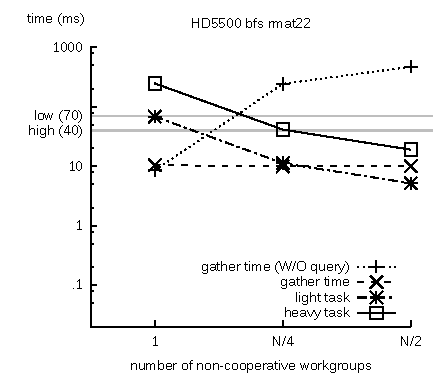
\includegraphics[width=.67\columnwidth]{hd5500_bfs_rmat22.pdf}
%\vspace{-2mm}
\caption{Example gather time and non-cooperative timing results}\label{fig:fine-grained-timing}
\vspace{-3mm}
\end{figure*}


\begin{table}
\normalsize
\centering
\begin{tabular}{ l l | l l | l l }
\multicolumn{2}{c|}{overall} & \multicolumn{2}{c|}{barrier} & \multicolumn{2}{c}{wk.steal.} \\
mean & max & mean & max & mean & max \\
\hline
$1.08$ & $1.37^{\ddagger}$ & $1.07$ & $1.37^{\ddagger}$ & $1.12$ & $1.23^{\diamond}$ \\
\end{tabular}\\
{\small
 $^{\ddagger}$sssp usa\_ny, $^{\diamond}$octree
}
%\vspace{-2mm}
\caption{Cooperative kernel slowdown w/o multitasking}
\label{tab:overhead}
\vspace{-8mm}
\end{table}



\myparagraph{Results}
\mytab\ref{tab:overhead} shows the geometric mean and
maximum slowdown across all applications and inputs, with averages and
maxima computed over 10 runs per benchmark. For the maximum slowdowns,
we indicate which application and input was responsible. The slowdown is
below 1.5 even in the worst case, and closer to 1 on average. We consider
these results encouraging, especially since the performance of our
prototype could clearly be improved upon in a native implementation.


\subsection{Multitasking via Cooperative Scheduling}\label{sec:responsiveness}

We now assess the responsiveness of multitasking between a
long-running cooperative kernel and a series of short, non-cooperative
kernel launches, and the performance impact of multitasking on the
cooperative kernel.

% In order to simulate non-persistent workloads alongside kernels of
% blocking algorithms, we use a matrix multiplication kernel where
% matrix dimensions are tuned to trigger the relevant execution
% duration.

\myparagraph{Experimental setup} For a given cooperative kernel and
its input, we launch the kernel and then repeatedly schedule a
non-cooperative kernel that aims to simulate the intensity of one of
the three classes of graphics rendering workload discussed in
\mysec\ref{sec:sizingnoncoop}. In practice, we use a matrix
multiplication kernel as the non-cooperative workload, with matrix
dimensions tailored to reach the appropriate execution duration.  We
conduct separate runs where we vary the number of workgroups requested
by the non-cooperative kernel, considering the cases where one, a
quarter, a half, and all-but-one, of the total number of workgroups
are requested. For the graph algorithms we try both
regular and query barrier implementations.

Our experiments span 13 pairs of cooperative kernels and inputs, 3
classes of non-cooperative kernel workloads, 4 quantities of
workgroups claimed for the non-cooperative kernel and 2 variations of
resizing barriers for graph algorithms, leading to 288 configurations.
We run each configuration 10 times, in order to report averaged
performance numbers. For each run, we record the execution time of the
cooperative kernel. For each scheduling of the non-cooperative kernel
during the run, we also record the \emph{gather time} needed by the
scheduler to collect enough workgroups to launch the non-cooperative
kernel, and the non-cooperative kernel execution time.
%
%We sanity-check
%whether all kernels perform their computations correctly by comparing
%their result with reference results.

%To work around compiler crash and compiler hang bugs in Intel's
%current OpenCL drivers, we had to apply some semantics-preserving
%changes to some applications.  Driver bugs also meant that we could
%not obtain results for some configurations where the non-cooperative
%kernel asks for all-but-one workgroups (namely bc, bfs, l-sssp, and
%color).  These configurations led to severe failures such as machine
%freezes and blue screens.

% Whenever a cooperative or non-cooperative kernel terminates, we verify
% that it has really performed its computation by comparing its results
% against the expected one. We encountered two kind of issues during the
% experiments: some configurations would lead to a system freeze or crash
% although they run fine on other GPUs. Although we don't claim that our
% programs are all correct, this issue seems to indicate a bug in the
% OpenCL compiler or driver of the problematic GPU. We also have some
% cooperative kernels that returned invalid results when the
% non-cooperative kernel takes all-but-one of the cooperative kernel
% workgroups, we decided to ignore these results.


\myparagraph{Responsiveness}
%
\myfiglong\ref{fig:fine-grained-timing} reports, on three
configurations, the average gather and execution times for the
non-cooperative kernel w.r.t. the quantity of workgroups allocated to
it.  A logarithmic scale is used for time since gather times tend to
be much smaller than execution times. The horizontal grey lines
indicates the desired period for non-cooperative kernels.  These
graphs show a representative sample of our results; the full set of
graphs for all configurations is provided in supplementary material.

The left most graph illustrates a work
stealing example.  When the non-cooperative kernel is given only one
workgroup, its execution is so long that it cannot complete within the
period required for a screen refresh. The gather time is very good
though, since the scheduler needs to collect only one workgroup.  The
more workgroups are allocated to the non-cooperative kernels, the
faster it can compute: here the non-cooperative kernel becomes fast
enough with a quarter (resp.\ half) of available workgroups for light
(resp.\ heavy) graphics workload. Inversely, the gather time increases
since the scheduler must collect more and more workgroups.

The middle and right graphs show results for graph algorithms.  These
algorithms use barriers, and we experimented with the regular and
query barrier implementations described in
\mysec\ref{sec:resizingbarrier}.  The execution times for the
non-cooperative task are averaged across all runs, including with both
types of barrier.  We show separately the average gather time
associated with each type of barrier.  The graphs show a similar trend
to the left-most graph: as the number of non-cooperative workgroups
grows, the execution time decreases and the gather time
increases.%\footnote{The right figure has only 3 points per line:
  %recall that for bfs there are no runs with ``all-but-one''
  %non-cooperative workgroups.}
%
the gather time is higher on the right figure: the rmat22 input graph
is rather wide than deep, so the graph algorithm reaches resizing
barriers less often than for the ecology input of the middle figure
for instance. The scheduler thus has fewer opportunities to collect
workgroups and gather time increases. Nonetheless, scheduling
responsiveness can benefit from the query barrier: when used, this
barrier lets the scheduler collect all needed workgroups as soon as
they hit a resizing barrier. As we can see, the gather time of the
query barrier is almost stable w.r.t.\ the number of workgroups that
needs to be collected.


\begin{figure}
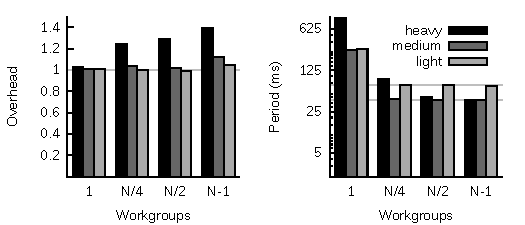
\includegraphics[width=\columnwidth]{heavy.pdf}
%\vspace{-2mm}
\caption{Performance impact of multitasking cooperative and non-cooperative workloads, and the period with which non-cooperative kernels execute}\label{fig:performance}
\vspace{-5mm}
\end{figure}


\myparagraph{Performance} \myfiglong\ref{fig:performance} reports the
overhead brought by the scheduling of non-cooperative kernels over the
cooperative kernel execution time.  This is the slowdown associated
with running the cooperative kernel in the presence of multitasking,
vs.\ running the cooperative kernel in isolation (geometric mean over
all applications and inputs).  We also show the period at which
non-cooperative kernels can be scheduled (arithmetic mean over all
applications and inputs).
We show results for the three workloads listed in
\mysec~\ref{sec:sizingnoncoop}. The two gray horizontal lines in the
period graph correspond to the period goals of the workloads: the
higher (resp. lower) line corresponds to a period of 70ms (resp. 40ms)
for the light (resp. medium and heavy) workload.

Co-scheduling non-cooperative kernels that request a single workgroup leads to almost no overhead, but the period is far too high to meet the needs
of any of our three workloads; e.g.\ a heavy workload averages a
period of 939 ms. As more workgroups are dedicated to non-cooperative
kernels, they execute quickly enough to be scheduled at the expected
period. For the light and medium workloads, a quarter
of the workgroups executing the non-cooperative kernel are able to meet
their goal period (70 and 40 ms resp.). However, a quarter of the
workgroups are not sufficient to meet the goal for the heavy workload
(giving a mean period of 88 ms). If half of the workgroups are
allocated to the non-cooperative kernel, the heavy workload averages $\sim$10\% over its goal period (mean of 44 ms). If all-but-one are allocated, the heavy workload reaches its goal period.
%
Yet, as expected, allocating more non-cooperative workgroups increases
the execution time of the cooperative kernel.

Still, heavy workloads meet their period by allocating all-but-one
non-cooperative workgroups, incurring a slow down of less than
1.4$\times$ on average. Light and medium workloads meet their period
with only a negligible overhead of the cooperative kernel (less than a
1.03$\times$ slowdown on average).

We consider these results encouraging, since they provide a lower
bound on potential performance of our cooperative kernels
model. Implementing the model natively, with device-specific runtime
support, could only improve performance and responsiveness compared
with that of our megakernel-based prototype.

\section{Related Work}\label{sec:relatedwork}

\myparagraph{Irregular algorithms and persistent kernels}
%
There has been a lot of work on accelerating blocking irregular
algorithms using GPUs, and on the \emph{persistent threads}
programming style for long-running
kernels~\cite{owens-persistent,DBLP:conf/ipps/KaleemVPHP16,DBLP:conf/ipps/DavidsonBGO14,DBLP:conf/hipc/HarishN07,DBLP:journals/topc/MerrillGG15,DBLP:conf/egh/VineetHPN09,DBLP:conf/ppopp/NobariCKB12,DBLP:conf/hpcc/SolomonTT10a,DBLP:conf/popl/PrabhuRMH11,DBLP:conf/ppopp/Mendez-LojoBP12,DBLP:conf/oopsla/PaiP16,DBLP:conf/oopsla/SorensenDBGR16,DBLP:conf/egh/CedermanT08,TPO10,BNP12,Pannotia}.
These approaches rely on the occupancy-bound execution model, flooding
available compute units with work, so that the GPU is unavailable for
other tasks, and assuming fair scheduling between occupant workgroups,
which is unlikely to be guaranteed on future GPU platforms.
%
As our experiments demonstrate, our cooperative kernels model allows blocking algorithms
to be upgraded to run in a manner that facilitates responsive multitasking.

%\vspace{-1mm}

\myparagraph{Preemptive multitasking on GPUs}
%
Hardware support for preemption has been proposed for \nvidia GPUs,
as well as \emph{SM-draining}
whereby workgroups occupying a symmetric multiprocessor (SM; a compute
unit using our terminology) are allowed to complete until the SM becomes free for
other tasks~\cite{DBLP:conf/isca/TanasicGCRNV14}.  SM draining is limited the presence of blocking constructs, since it may not be possible to drain a blocked workgroup.
%
A follow-up work adds the notion of SM \emph{flushing},
where a workgroup can be re-scheduled
from scratch if it has not yet committed side-effects~\cite{DBLP:conf/asplos/ParkPM15}.  Both approaches have been evaluated
using simulators, over sets of regular GPU kernels.  Very recent \nvidia GPUs support
preemption, though it is not clear whether they guarantee fairness~\cite{PascalWhitepaper}.

The advantages of preemption are that it does not require programmer
effort, and guards against a rogue long-running kernel making the GPU
unavailable for other tasks.  The main drawback is that \emph{every}
kernel takes a potential performance hit.
%
If implemented natively, our solution does not impact performance on regular kernels that are not scheduled with cooperative kernels.
Furthermore, careful placement of
our new primitives can exploit problem structure, enabling more efficient multitasking than
application-oblivious preemption.  There is scope for combining the approaches: if a
cooperative kernel is insufficiently cooperative, hardware support for preemption could
be invoked to prevent the kernel from denying other tasks access to
the GPU indefinitely.

%\vspace{-1mm}


\myparagraph{Optimizing GPU scheduling}
%
A number of works have considered how best to schedule dynamic
workloads on GPUs~\cite{DBLP:journals/tog/SteinbergerKKHKS12,DBLP:conf/ics/WuCLSV15,DBLP:conf/usenix/KatoLRI11,DBLP:journals/tog/SteinbergerKBKDS14,DBLP:journals/rts/ElliottA12,DBLP:conf/sosp/RossbachCSRW11}.  Among these, the Whippletree approach employs a persistent
megakernel to schedule multiple, dynamic tasks in a manner that aims
to best utilise GPU
resources~\cite{DBLP:journals/tog/SteinbergerKBKDS14}, and the TimeGraph
approach similarly aims to optimise scheduling of competing workloads,
in the context of OpenGL~\cite{DBLP:conf/usenix/KatoLRI11}.
None of these approaches tackle
the problem of \emph{fair} scheduling on GPUs, thus they do not aid in safe deployment of blocking irregular algorithms.

CUDA and OpenCL provide the facility for a kernel to spawn further
kernels~\cite{cuda-75}.  This \emph{dynamic parallelism}
can be used to implement a GPU-based scheduler, by having an initial
scheduler kernel repeatedly spawn further kernels as required,
according to some scheduling
policy~\cite{DBLP:conf/ppopp/Muyan-OzcelikO16}.  However, kernels that
uses dynamic parallelism are still prone to unfair scheduling of
workgroups, and thus does not help in deploying blocking algorithms on
GPUs.

\myparagraph{Cooperative multitasking}
%
Cooperative multitasking was offered in older operating systems
(e.g. pre 1995 Windows) and is still used by some operating systems,
such as RISC OS~\cite{risc-os-multitasking}.

%Many programming
%languages offer cooperative multitasking via variations of
%co-routines, e.g. co-routine objects in Python
%\footnote{\url{https://docs.python.org/3/reference/datamodel.html\#coroutine-objects}}
%and Lua,
%\footnote{\url{https://www.lua.org/pil/9.1.html}}
%and Ruby's
%\emph{fiber}.
%\footnote{\url{http://ruby-doc.org/core-2.1.1/Fiber.html}}

In the context of GPUs, cooperative multitasking has been used to
refer to the standard programming model, where the onus is on the GPU kernel
to complete execution within a reasonable time budget~\cite{adriaens2012case,CPE:CPE1722}.
%
This is in contrast to our cooperative kernels, which specifically aim to support the needs of long-running GPU tasks.

%\vspace{-1mm}

\section{Conclusions and Future Work}\label{sec:conclusion}

We have proposed \emph{cooperative kernels}, a small set of GPU
programming extensions that allow long-running, blocking kernels to be
fairly scheduled and to share GPU resources with other workloads.
Experimental results using our megakernel-based prototype \cutthree{over three Intel GPUs}
shows that the model is a good fit for the needs of current
GPU-accelerated irregular algorithms.  The
performance that could be gained through a native implementation with
dedicated driver support would be even better.
%
Avenues for future work include seeking
additional classes of irregular algorithms to which the model might
(be extended to) apply (to), investigating implementing native support
in open source drivers, and integrating
cooperative kernels into template- and compiler-based programming
models for graph algorithms on
GPUs~\cite{DBLP:conf/ppopp/WangDPWRO16,DBLP:conf/oopsla/PaiP16}.
%  As more vendors
%adopt the advanced features of OpenCL that our approach requires, we
%will be in a position to assess the programming model across a wider
%range of devices.

\clearpage

\bibliographystyle{abbrvnat}
\bibliography{tyler}

\iffalse


\clearpage

\appendix

\section{Operational Semantics for Cooperative Kernels}\label{appendix:semantics}

\newcommand{\myss}{\mathit{ss}}
\newcommand{\Stmts}{\mathsf{Stmts}}
\newcommand{\threadstates}{\mathsf{ThreadStates}}
\newcommand{\sharedstates}{\mathsf{SharedStates}}
\newcommand{\sync}{\mathsf{sync}}

In \mysec\ref{sec:semantics} we presented the semantics of cooperative
kernels relatively informally, using English, to provide the intuition
behind our programming model.  We now back this up with a more formal
presentation as an operational semantics for an abstract GPU
programming model.

\myparagraph{States}
%
Let $L$ be a set of \emph{local states} that abstractly captures the
private memory associated with a thread executing a GPU kernel.  Let
$\Stmts$ denote the set of all possible statements that a
thread can execute.  We do not detail the structure of these
statements, except that we assume sequential composition of statements
is provided by the $\code{;}$ separator, and that the $\offerkill$,
$\offerfork$, $\globalbarrier$ and $\resizingglobalbarrier$ primitives
from our cooperative kernels programming model are valid statements.

A \emph{thread state} is then a pair $(l, \myss)$, where $l \in L$ and
$\myss \in \Stmts$.  The $l$ component captures the valuation of all the
thread's private memory, and the $\myss$ component captures the
remaining statements to be executed by the thread.  Let $\threadstates$ denote the set of all thread states.

Assuming that $d > 0$ threads per workgroup were requested on kernel launch, a \emph{workgroup state}
is a $d$-tuple $((l_0, \myss_0), \dots, (l_{d-1}, \myss_{d-1}))$, where each $(l_i, \myss_i)$ is the thread state for the $i$th thread in the workgroup $(0\leq i < d$).

Assuming that $N > 0$ was specified as the maximum number of
workgroups that should execute the cooperative kernel, a \emph{kernel
  state} is then a pair
%
\[
(\sigma, (w_0, \dots, w_{M-1}, \underbrace{\bot, \dots,
\bot}_{N-M}))\]
%
where: $\sigma$ represents the shared state of the kernel; $M \leq N$
is the number of \emph{active} workgroups; $w_i$ is the workgroup
state for active workgroup $i$ ($0 \leq i < M$); and $N-M$ occurrences
of $\bot$ indicate \emph{absent} workgroups.  Let $\sharedstates$
denote the set of all possible shared states.  We regard
workgroup-local storage as being part of the shared state of a kernel.

\myparagraph{Thread-level transitions}
%
We leave the semantics for thread-level transitions abstract, assuming
a binary relation $\rightarrow_{tau}$ on $\sharedstates{} \times
\threadstates{}$.  If $(\sigma, (l, \myss)) \rightarrow_{\tau}
(\sigma', (l', \myss'))$, this indicates that if a thread is in local
state $(l, \myss)$, the thread can transition to local state $(l',
\myss')$, changing the shared state from $\sigma$ to $\sigma'$ in the
process.

All we require is that $(\sigma, (l, \myss)) \rightarrow_{\tau}
(\sigma', (l', \myss'))$ if $\myss$ has the form $\mathsf{special}();
\mathit{tt}$, where $\mathsf{special}$ is one of $\offerkill$,
$\offerfork$, $\globalbarrier$ or $\resizingglobalbarrier$.  This is
because we shall specifically define the meaning of the new primitives
introduced by our programming model.

\myparagraph{Memory synchronisation}
%
GPUs are known to have relaxed memory models~\cite{ABDGKPSW-2015}.  To abstractly
account for this, we assume that the shared state component $\sigma$
is not simply a mapping from locations to values, but instead
captures all the intricacies of GPU memory that can lead to this
relaxed behaviour.  We also assume a function $\sync$ which, given a
kernel state $\kappa$, returns a set of kernel states.  The idea is
that each $\kappa' \in \sync(\kappa)$ is a possible kernel state that
can be reached from $\kappa$ by stalling until all stores to memory
and loads from memory to thread-local storage have completed.  All we
require is that $\sync$ does not modify the number of active
workgroups nor the component of a thread state that determines which
statements remain to be executed.

\begin{figure*}
\begin{center}

\[
\inferrule{
w_i(j) = (l, \myss)
\\
(\sigma, (l, \myss)) \rightarrow_{\tau} (\sigma', (l', \myss'))
\\
w_i' = w_i[j \mapsto (l', \myss')]
}
{
(\sigma, (\dots, w_i, \dots)) \rightarrow (\sigma', (\dots, w_i', \dots))
}
(\textsc{Thread-Step})
\]

\medskip

\[
\inferrule{
\forall j \;.\; w_i(j) = (l_j, \offerkill();\myss)
\\
w_i' = ((l_0, \myss), \dots, (l_{d-1}, \myss))
}
{
(\sigma, (\dots, w_i, \dots)) \rightarrow (\sigma, (\dots, w_i', \dots))
}
(\textsc{Kill-No-Op})
\]

\medskip

\[
\inferrule{
\forall j \;.\; w_{M-1}(j) = (l_j, \offerkill();\myss)
\\
M > 0
}
{
(\sigma, (\dots, w_{M-2}, w_{M-1}, \bot, \dots, \bot)) \rightarrow (\sigma, (\dots, w_{M-2}, \bot, \bot, \dots, \bot))
}
(\textsc{Kill})
\]

\medskip

\[
\inferrule{
\forall j \;.\; w_i(j) = (l_j, \offerfork();\myss)
\\
w_i' = ((l_{0}, \myss), \dots, (l_{d-1}, \myss))
\\
k \in [0, N - M]
\\
\forall a \in [0, k - 1] \;.\; w_{M+a} = ((l_{0}, \myss), \dots, (l_{0}, \myss))
}
{
(\sigma, (\dots, w_i, \dots, w_{M-1}, \bot, \dots, \bot)) \rightarrow (\sigma, (\dots, w_i', \dots, w_{M-1}, w_{M}, \dots, w_{M+k-1}, \bot, \dots, \bot))
}
(\textsc{Fork})
\]

\medskip

\[
\inferrule{
\forall i \;.\;\forall j\;.\;w_i(j) = (l_{i,j}, \globalbarrier();\myss)
\\
\forall i \;.\;\forall j\;.\;w_i'(j) = (l_{i,j}, \myss)
\\\\
\kappa \in \sync((\sigma , (w_{0}', \dots, w_{M-1}', \bot, \dots, \bot))
}
{
(\sigma, (w_{0}, \dots, w_{M-1}, \bot, \dots, \bot)) \rightarrow \kappa
}
(\textsc{Barrier})
\]

\medskip

\[
\inferrule{
\forall i \;.\;\forall j\;.\;w_i(j) = (l_{i,j}, \resizingglobalbarrier();\myss)
\\
\forall j\;.\;w_{0}'(j) = (l_{1,j}, \globalbarrier(); \offerfork(); \globalbarrier(); \globalbarrier();\myss)
\\
\forall i \neq 1 \;.\;\forall j\;.\;w_i'(j) = (l_{i,j}, \globalbarrier(); \globalbarrier(); \offerkill(); \globalbarrier();\myss)
}
{
(\sigma, (w_{0}, \dots, w_{M-1}, \bot, \dots, \bot)) \rightarrow (\sigma, (w_{0}', \dots, w_{M-1}', \bot, \dots, \bot))
}
(\textsc{Resizing-Barrier})
\]

\end{center}

\caption{Abstract operational semantics for our cooperative kernels language extensions}\label{fig:semanticrules}

\end{figure*}

\myparagraph{Operational semantics rules}
%
\myfiglong\ref{fig:semanticrules} presents the rules of our
operational semantics, defining a relation $\rightarrow$ on kernel
states.

Rule $\textsc{Thread-Step}$ defines the semantics for thread making a
single execution step, delegating to the abstract $\rightarrow_{\tau}$
relation to determine how the thread's local state and the shared
state component change.  For simplicity, this rule ignores the
semantics of intra-workgroup barriers, which are not our focus here.

Rule $\textsc{Kill-No-Op}$ reflects the fact that when a workgroup
reaches $\offerkill$, this can always be treated as a no-op.  Whether
a scheduler implementation accepts $\offerkill$ calls or not depends
on competing workloads and how the scheduler has been designed to meet
the non-functional requirements discussed in
\mysec\ref{sec:nonfunctional}, but in general the programmer should
always be prepared for the possibility that a workgroup survives after
calling $\offerkill$.

The case where a workgroup's offer to be killed is accepted by the
scheduler is captured by rule $\textsc{Kill}$.  Because we have
adopted a semantics where workgroup 0 is never killed and where only
the workgroup with the highest id can be killed, the rule only fires
if $M > 0$ and workgroup $M-1$ has reached $\offerkill$.  The rule has
the effect of replacing the workgroup state for $w_{M-1}$
with $\bot$.

Recall that $\offerkill$ is a workgroup-level function: the same
syntactic $\offerfork$ call must be reached by all threads in a
workgroup.  This is captured in our rules by requiring in both
$\textsc{Kill-No-Op}$ and $\textsc{Kill}$ that every thread is ready
to execute $\offerkill$ followed by an identical statement $\myss$.
Neither rule applies until all threads in a workgroup reach
$\offerfork$, and the workgroup gets stuck if multiple threads in a
workgroup reach $\offerfork$ with different subsequent statements.

The $\textsc{Fork}$ rule similarly requires all threads in a workgroup
to reach $\offerfork$ with identical following statements.  A
nondeterministic number of new workgroups, $k$, is selected to be
forked, where $k \in [0, N-M]$.  Importantly, $k=0$ is always a
legitimate choice, in which case $\offerfork$ has no effect on the
number of workgroups that are executing.  In the case where $k > 0$,
$k$ new workgroup states are created, where each workgroup inherits
the local state of thread 0 in $w_i$, the workgroup executing the fork
call.  After $\offerfork$, all threads in all workgroups, including
the new threads, proceed to execute the sequence of statements $\myss$
that followed $\offerfork$.

A simplification here is that we do not model transmission of
particular annotated variables from thread 0 of the forking workgroup,
instead specifying that the entire local state of the workgroup is
transmitted.  Extending the semantics to transmit only annotated
variables would be straightforward but verbose, requiring the local
memory component of a thread state to be split into two: the part of
the local state to be transmitted (modelling $\transmit$-annotated
variables), and the rest of the local state.

The $\textsc{Barrier}$ rule requires that \emph{every} thread
executing the kernel reaches $\globalbarrier$ an identical following
statement.  This reflects that fact that $\globalbarrier$ is a
kernel-level function.  Each thread then skips over the
$\globalbarrier$ call, and the $\sync$ function is applied to yield
a set of kernel states that can arise due to memory synchronization
taking place.  An arbitrary member of this set is selected as the next
kernel state.

Despite its apparent complexity, the $\textsc{Resizing-Barrier}$ rule simply implements the rewriting of $\resizingglobalbarrier$ in terms of $\globalbarrier$, $\offerkill$ and $\offerfork$ discussed in \mysec\ref{sec:semantics}.


\section{Alternative Semantic Choices}\label{appendix:semanticalternatives}

The semantics of cooperative kernels has been guided by the practical
applications we have studied (described in
\mysec\ref{sec:portingalgorithms}).  We now discuss several cases
where we might have taken different and also reasonable semantic
decisions.

\myparagraph{Killing order}
%
We opted for a semantics whereby only the active workgroup with the
highest id can be killed.  This has an appealing property: it means
that the ids of active workgroups are contiguous, which is important
for processing of contiguous data.  The cooperative graph traversal
algorithm of \myfig\ref{fig:cgraphsearch} illustrates this: the
algorithm is prepared for $\getglobalsize$ to change after each
resizing barrier call, but depends on the fact that $\getglobalid$
returns a contiguous range of thread ids.

A disadvantage of this decision is that it may provide sub-optimal
responsiveness from the point of view of the scheduler.  Suppose the
scheduler requires an additional compute unit, but the active thread
with the largest id is processing some computationally intensive work
and will take a while to reach $\offerkill$.  Our semantics means that
the scheduler cannot take advantage of the fact that another active
workgroup may invoke $\offerkill$ sooner.

Cooperative kernels that do not require contiguous thread ids might me
more suited to a semantics in which workgroups can be killed in any
order, but where workgroup ids (and thus thread global ids) are not
guaranteed to be contiguous.

\myparagraph{Keeping one workgroup alive}
%
Our semantics dictate that the workgroup with id 0 will not be killed
if it invokes $\offerkill$.  This avoids the possibility of the
cooperative kernel terminating early due to the programmer
inadvertently allowing all workgroups to be killed, and the decision
to keep workgroup 0 alive fits well with our choice to kill workgroups
in descending order of id.

However, there might be a use case for a cooperative kernel reaching a
point where it would be acceptable for the kernel to exit, although
desirable for some remaining computation to be performed if competing
workloads allow it.  In this case, a semantics where all workgroups can be killed via $\offerkill$ would be appropriate, and the programmer would need to guard each $\offerkill$ with an id check in cases where killing all workgroups would be unacceptable.  For example:
%
\lstset{basicstyle=\tt,numbers=none}
\begin{lstlisting}
  if($\getgroupid{0}$ != 0) $\offerkill$();
\end{lstlisting}
\lstset{basicstyle=\scriptsize\tt,numbers=left}
%
would ensure that at least workgroup 0 is kept alive.

\myparagraph{Transmission of partial state from a single thread}
%
Recall from the semantics of $\offerfork$ that newly forked workgroups
inherit the variable valuation associated with thread 0 of the forking
workgroup, but only for $\transmit$-annotated variables.  Alternative
choices here would be to have forked workgroups inherit values for
\emph{all} variables from the forking workgroup, and to have thread
$i$ in the forking workgroup provide the valuation for thread $i$ in
each spawned workgroup, rather than having thread 0 transmit the
valuation to all new threads.

We opted for transmitting only selected variables based on the
observation that many of a thread's private variables are dead at the
point of issuing $\offerfork$ or $\resizingglobalbarrier$, thus it
would be wasteful to transmit them.  A live variable analysis could
instead be employed to over-approximate the variables that might be
accessed by newly arriving workgroups, so that these are automatically
transmitted.

In all cases, we found that a variable that needed to be transmitted
had the property of being uniform across the workgroup.  That is,
despite each thread having its own copy of the variable, each thread
is in agreement on the variable's value.  As an example, the
$\keyword{level}$, $\keyword{in\_nodes}$ and $\keyword{out\_nodes}$
variables used in \myfig\ref{fig:cgraphsearch} are all stored in thread-private
memory, but all threads in a workgroup agree on the values of these
variables at each $\resizingglobalbarrier$ call.  As a result,
transmitting the thread 0's valuation of the annotated variables is
equivalent to (and more efficient than) transmitting values on a
thread-by-thread basis.  We have not yet encountered a real-world
example where our current semantics would not suffice.


\section{Graphs for Multitasking Experiments}\label{appendix:extragraphs}

We present the full set of graphs exemplified by the examples in
\myfig\ref{fig:fine-grained-timing}; for completeness we reproduce
those graphs here too.

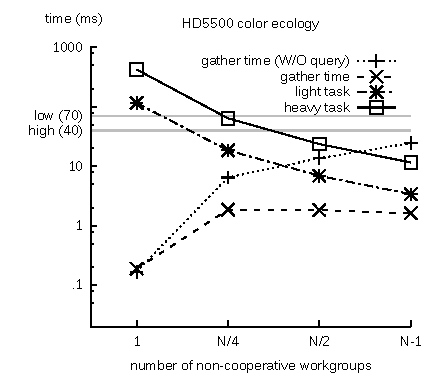
\includegraphics[width=.7\columnwidth]{images/barrier/hd5500_color_ecology.pdf} \\
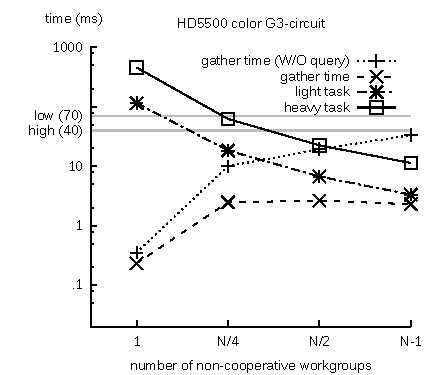
\includegraphics[width=.7\columnwidth]{images/barrier/hd5500_color_G3_circuit.pdf} \\
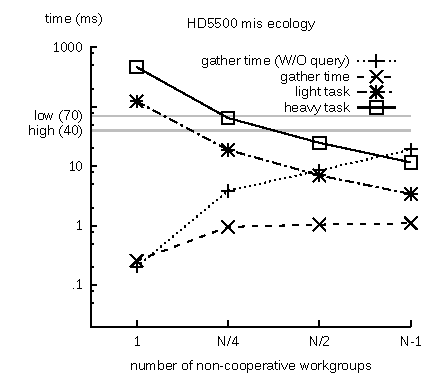
\includegraphics[width=.7\columnwidth]{images/barrier/hd5500_mis_ecology.pdf} \\
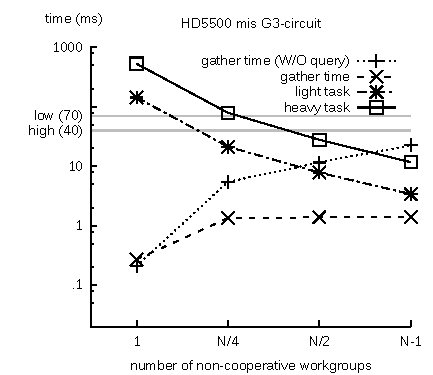
\includegraphics[width=.7\columnwidth]{images/barrier/hd5500_mis_G3_circuit.pdf} \\
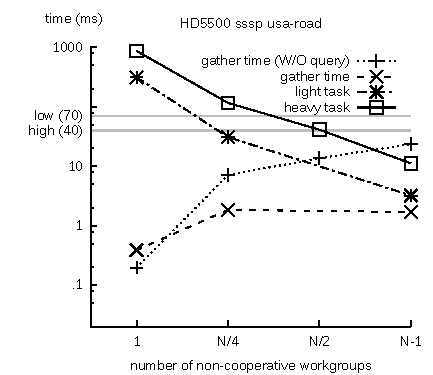
\includegraphics[width=.7\columnwidth]{images/barrier/hd5500_sssp_usa_road.pdf} \\
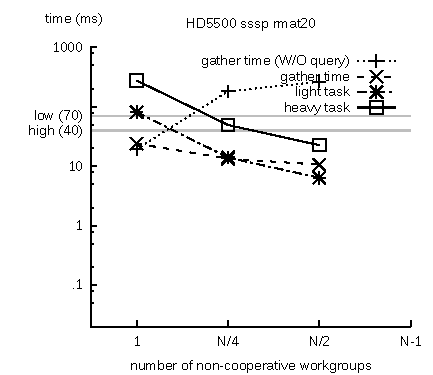
\includegraphics[width=.7\columnwidth]{images/barrier/hd5500_sssp_rmat20.pdf} \\
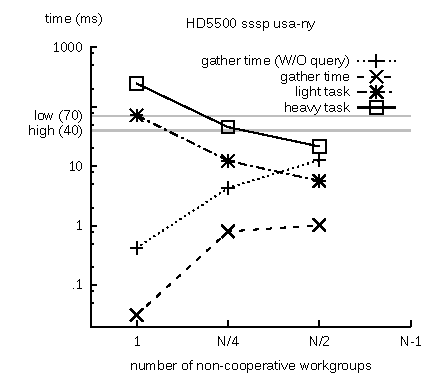
\includegraphics[width=.7\columnwidth]{images/barrier/hd5500_sssp_usa_ny.pdf} \\
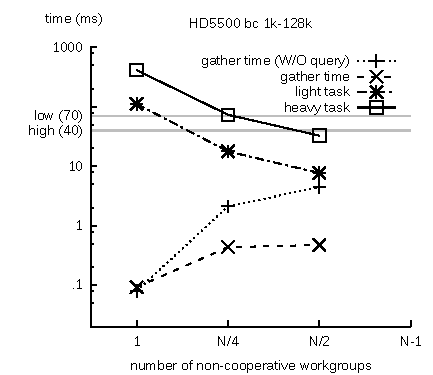
\includegraphics[width=.7\columnwidth]{images/barrier/hd5500_bc_1k_128k.pdf} \\
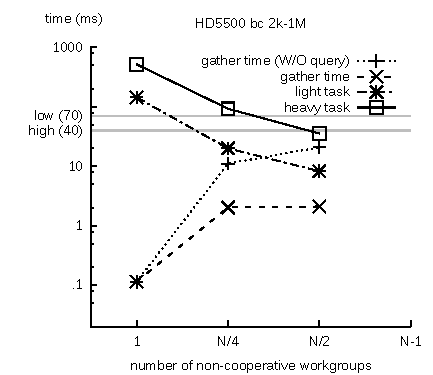
\includegraphics[width=.7\columnwidth]{images/barrier/hd5500_bc_2k_1M.pdf} \\
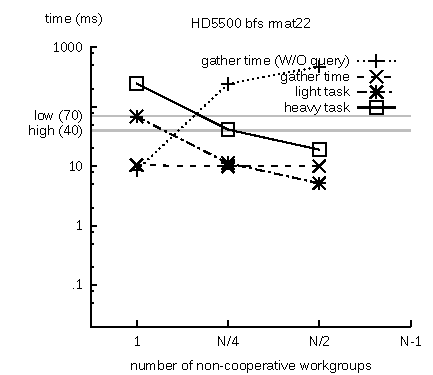
\includegraphics[width=.7\columnwidth]{images/barrier/hd5500_bfs_rmat22.pdf} \\
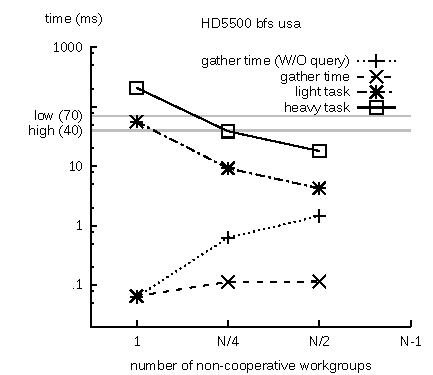
\includegraphics[width=.7\columnwidth]{images/barrier/hd5500_bfs_usa.pdf} \\
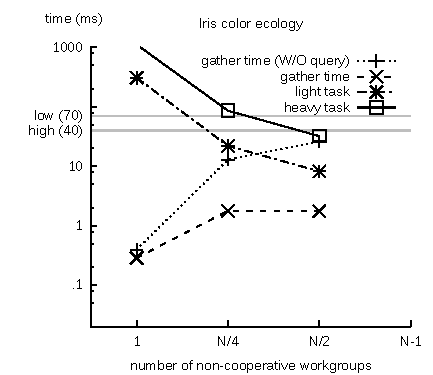
\includegraphics[width=.7\columnwidth]{images/barrier/iris_color_ecology.pdf} \\
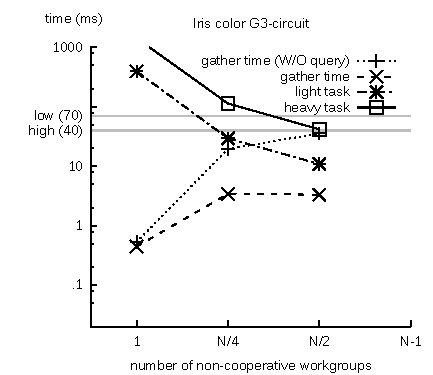
\includegraphics[width=.7\columnwidth]{images/barrier/iris_color_G3_circuit.pdf} \\
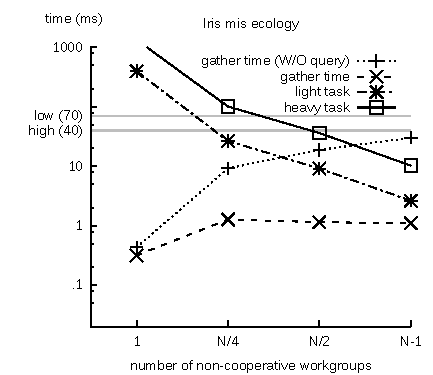
\includegraphics[width=.7\columnwidth]{images/barrier/iris_mis_ecology.pdf} \\
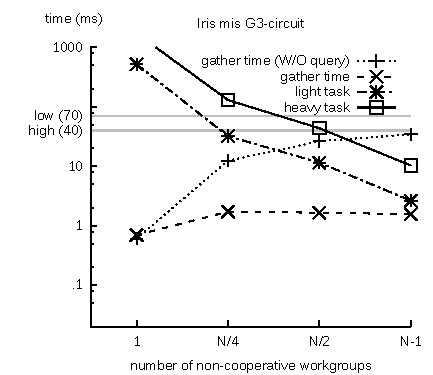
\includegraphics[width=.7\columnwidth]{images/barrier/iris_mis_G3_circuit.pdf} \\
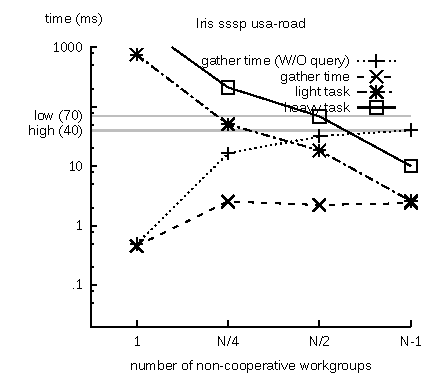
\includegraphics[width=.7\columnwidth]{images/barrier/iris_sssp_usa_road.pdf} \\
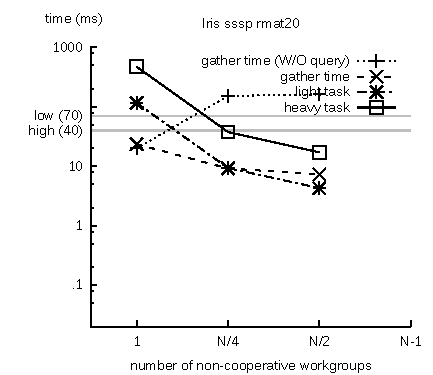
\includegraphics[width=.7\columnwidth]{images/barrier/iris_sssp_rmat20.pdf} \\
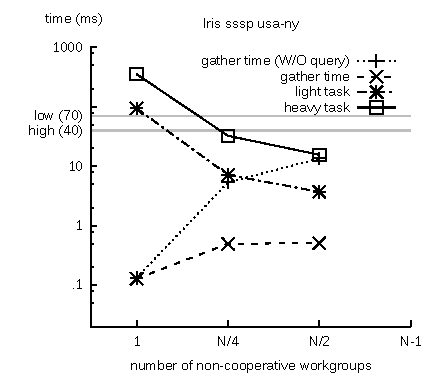
\includegraphics[width=.7\columnwidth]{images/barrier/iris_sssp_usa_ny.pdf} \\
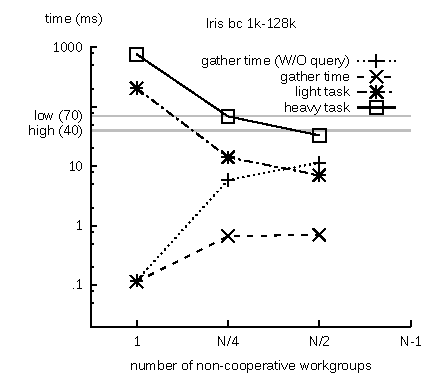
\includegraphics[width=.7\columnwidth]{images/barrier/iris_bc_1k_128k.pdf} \\
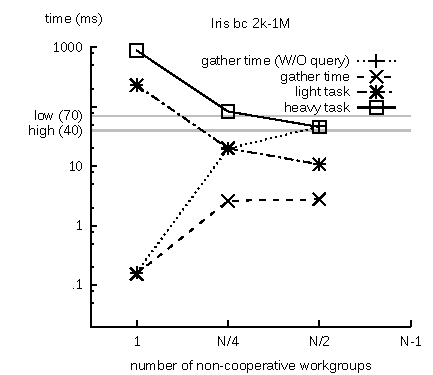
\includegraphics[width=.7\columnwidth]{images/barrier/iris_bc_2k_1M.pdf} \\
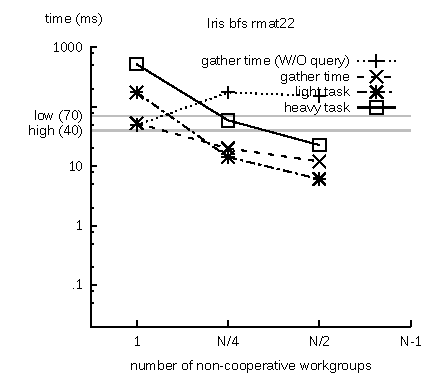
\includegraphics[width=.7\columnwidth]{images/barrier/iris_bfs_rmat22.pdf} \\
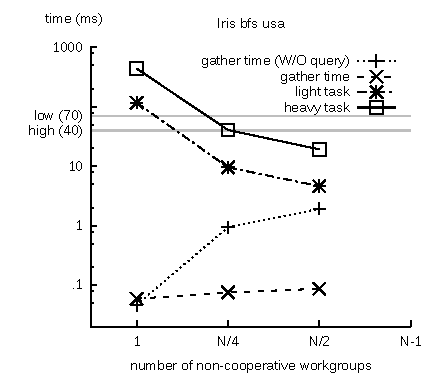
\includegraphics[width=.7\columnwidth]{images/barrier/iris_bfs_usa.pdf} \\
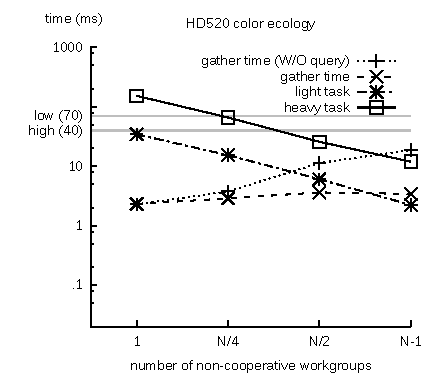
\includegraphics[width=.7\columnwidth]{images/barrier/hd520_color_ecology.pdf} \\
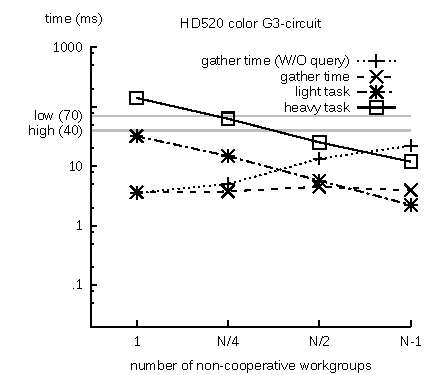
\includegraphics[width=.7\columnwidth]{images/barrier/hd520_color_G3_circuit.pdf} \\
\includegraphics[width=.7\columnwidth]{images/barrier/hd520_mis_ecology.pdf} \\
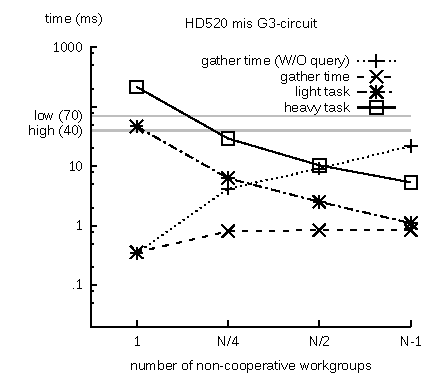
\includegraphics[width=.7\columnwidth]{images/barrier/hd520_mis_G3_circuit.pdf} \\
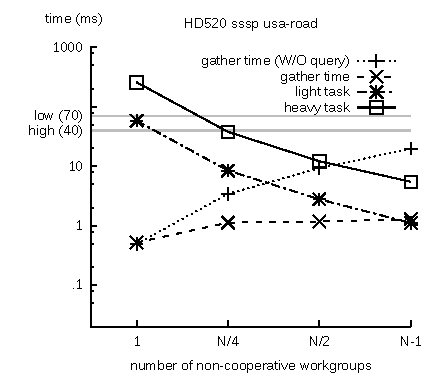
\includegraphics[width=.7\columnwidth]{images/barrier/hd520_sssp_usa_road.pdf} \\
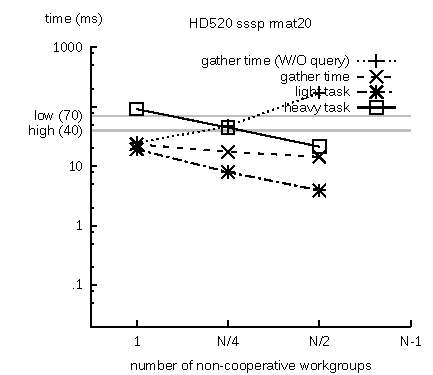
\includegraphics[width=.7\columnwidth]{images/barrier/hd520_sssp_rmat20.pdf} \\
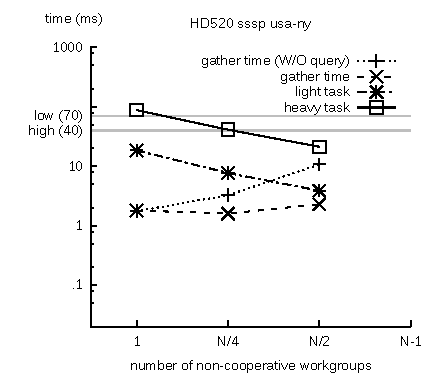
\includegraphics[width=.7\columnwidth]{images/barrier/hd520_sssp_usa_ny.pdf} \\
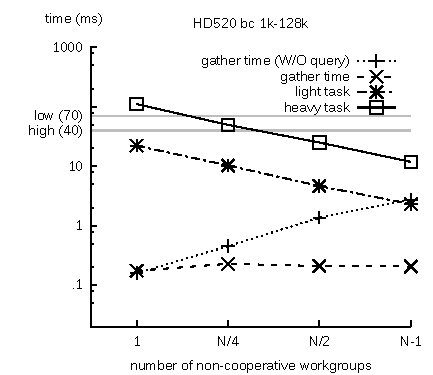
\includegraphics[width=.7\columnwidth]{images/barrier/hd520_bc_1k_128k.pdf} \\
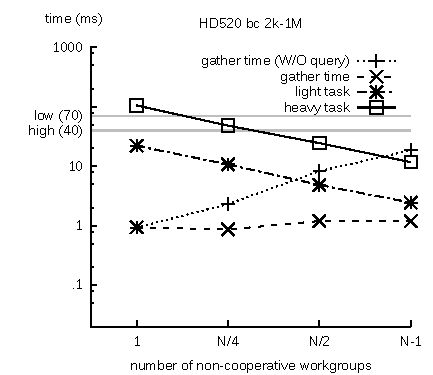
\includegraphics[width=.7\columnwidth]{images/barrier/hd520_bc_2k_1M.pdf} \\
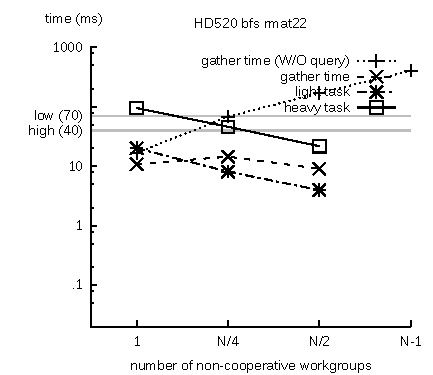
\includegraphics[width=.7\columnwidth]{images/barrier/hd520_bfs_rmat22.pdf} \\
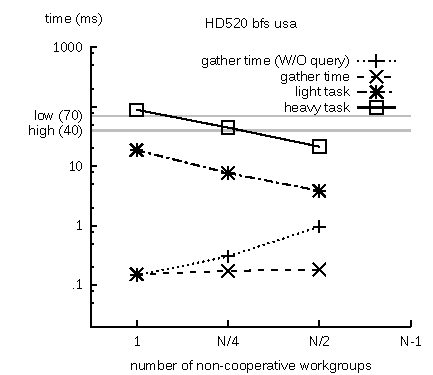
\includegraphics[width=.7\columnwidth]{images/barrier/hd520_bfs_usa.pdf} \\
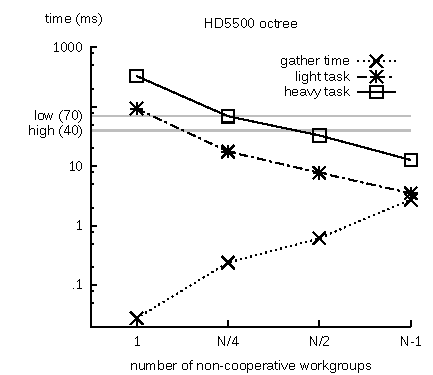
\includegraphics[width=.7\columnwidth]{images/ws/hd5500_octree_NA.pdf} \\
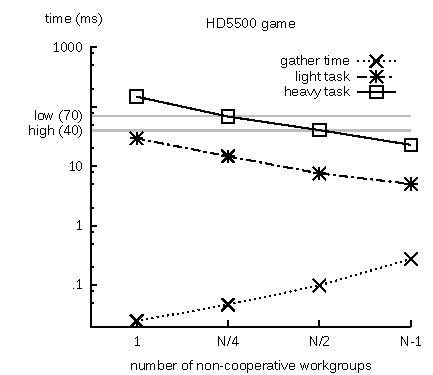
\includegraphics[width=.7\columnwidth]{images/ws/hd5500_connect_four_NA.pdf} \\
\includegraphics[width=.7\columnwidth]{images/ws/iris_octree_NA.pdf} \\
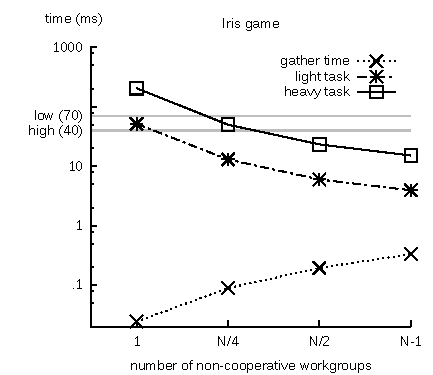
\includegraphics[width=.7\columnwidth]{images/ws/iris_connect_four_NA.pdf} \\
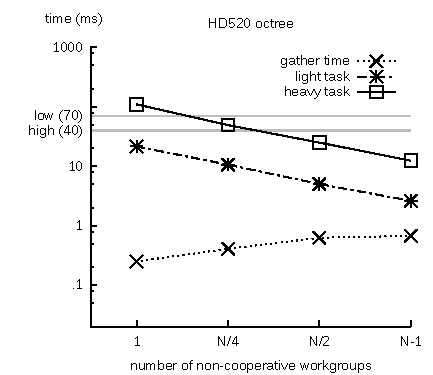
\includegraphics[width=.7\columnwidth]{images/ws/hd520_octree_NA.pdf} \\

\fi
\end{document}
